\apendice{Especificación de Requisitos}

\section{Introducción}
A continuación, se detallan los requisitos con los que cumplen la APIs desarrolladas que servirán de base también para la futura implementación de la aplicación móvil.
A este respecto, se siguieron las recomendaciones y lineamientos establecidos por norma IEEE 830-1998, que indica las características que debe tener un documento de especificación de requisitos de software \cite{ieee_830_1998_recommended}; a saber:

\begin{itemize}
\tightlist
\item
  \textbf{Corrección}: Todo requisito contenido en el documento, e implementado en el sistema, es válido si responde a un necesidad real, conduciendo al desarrollo de un sistema deseado.\\
\item
  \textbf{No ambiguo}: Cada requisito debe ser detallado de forma explícita y no prestarse a múltiples interpretaciones. \\
\item
  \textbf{Completo}: Todos los requisitos relevantes están contenidos en el documento de especificación de requisitos del sistema. \\
\item
  \textbf{Consistente}: No puede existir contradicción entre los requisitos del sistema, porque dicha situación imposibilitaría su implementación. \\
\item
  \textbf{Clasificado}: No todos los requisitos tienen el mismo nivel de relevancia para el sistema, por lo que éstos deben clasificarse bien sea según su importancia o por su estabilidad, lo cual permitirá enfocar los recursos en donde realmente se necesitan. \\
\item
  \textbf{Verificable}: El documento es verificable si sus requisitos se pueden poner a prueba de forma experimental a través de un proceso definido y no costoso que ayude a validar su funcionamiento. \\
\item
  \textbf{Modificable}: El documento debe estar estructurado de tal forma que puedan efectuarse cambios en los requisitos de manera fácil, completa y consistente. \\
\item
  \textbf{Trazable}: Se debe conocer el origen de cada requisito al mismo tiempo que se referencia cada uno a los componentes de diseño e implementación. \\
\end{itemize}

\section{Objetivos generales}

El presente proyecto persigue los siguientes objetivos generales en cuanto a las características que debe cumplir el backend: 

\begin{itemize}
    \item Ser eficiente y eficaz para el procesamiento y manipulación de datos.
    \item Presentar una sólida, coherente y confiable lógica de negocio. 
    \item Ponderar la seguridad, privacidad e integridad de la información sensible que los usuarios comparten.
    \item Permitir una robusta escalabilidad y rendimiento del sistema.
    \item Permitir que el sistema se integre con servicios internos y externos tales como APIs.
    \item Habilitar un monitoreo y un registro de errores que haga al sistema tolerante a fallos. 
\end{itemize}

\section{Catálogo de requisitos}

\begin{itemize}
\tightlist
\item
  \textbf{RF-1 Gestión de usuarios:} La API debe permitir el manejo de usuarios.\\
  \begin{itemize}
  \tightlist
  \item
    \textbf{RF-1.1 Registro de usuario:} Permite al usuario registrarse en el sistema.\\
  \item
    \textbf{RF-1.2 Autenticación del usuario:} Permite al usuario ingresar al sistema.\\
  \item
    \textbf{RF-1.3 Actualización del usuario:} Permite al usuario actualizar sus datos en el sistema.\\
  \item
    \textbf{RF-1.4 Obtener información del usuario:} Permite al usuario ver todos sus datos registrados.\\
  \item
    \textbf{RF-1.5 Actualizar estado de activación del usuario:} Permite a un administrador desactivar un usuario.\\
  \item
    \textbf{RF-1.6 Actualizar estado de baneo del usuario:} Permite negar el acceso a un usuario debido a conducta sospechosa.\\
\end{itemize}    
\end{itemize}

\begin{itemize}
\tightlist
\item
  \textbf{RF-2 Gestión de artículos:} La API debe permitir el manejo de artículos.\\
  \begin{itemize}
  \tightlist
  \item
    \textbf{RF-2.1 Crear artículo:} Permite al usuario administrador crear artículos. \\
    \begin{itemize}
    \tightlist
    \item
      \textbf{RF-2.2.1: Agregar categoría a un artículo:} El usuario administrador debe poder agregar una categoría al artículo.\\
    \item
      \textbf{RF-2.2.2: Eliminar categoría a un artículo:} El usuario administrador debe poder eliminar una categoría al artículo. \\
    \end{itemize}
  \item
    \textbf{RF-2.2 Obtener artículos:} Permite a todos los usuarios obtener un listado de todos los artículos.\\
  \item
    \textbf{RF-2.3 Actualización de un artículo:} Permite al usuario administrador actualizar un artículo.\\
  \item
    \textbf{RF-2.4 Eliminar un artículo:} Permite al usuario administrador eliminar un artículo\\
\end{itemize}    
\end{itemize}

\begin{itemize}
\tightlist
\item
  \textbf{RF-3 Gestión de categorías:} La API debe permitir gestionar categorías para poder categorizar los contenidos.\\
  \begin{itemize}
  \tightlist
  \item
    \textbf{RF-3.1 Crear categoría:} Permite al usuario administrador crear categorías. \\
  \item
    \textbf{RF-3.2 Obtener categorías:} Permite a todos los usuarios obtener un listado de todos los artículos.\\
  \item
    \textbf{RF-3.3 Actualizar categorías:} Permite al usuario administrador actualizar una categoría.\\
  \item
    \textbf{RF-3.4 Eliminar categorías:} Permite al usuario administrador eliminar un categoría. \\
\end{itemize}    
\end{itemize}

\begin{itemize}
\tightlist
\item
  \textbf{RF-4 Gestión de Preguntas y Respuestas:} La API debe a permitir a los usuarios realizar preguntas y responder dudas sobre la EM.\\
  \begin{itemize}
  \tightlist
  \item
    \textbf{RF-4.1 Crear preguntas:} Permite al usuario crear preguntas. \\
  \item
    \textbf{RF-4.2 Obtener preguntas:} Permite a todos los usuarios obtener un listado de todas las preguntas.\\
      \item
    \textbf{RF-4.3 Responder a preguntas:} Permite a todos los usuarios responder a preguntas.\\
          \item
    \textbf{RF-4.4 Obtener preguntas a respuestas:} Permite a todos los usuarios obtener todas las preguntas y sus respuestas asociadas.\\
    \end{itemize}    
\end{itemize}

\begin{itemize}
\tightlist
\item
  \textbf{RF-5 Gestión recetas:} La API debe permitir a los usuarios administradores crear recetas.\\
  \begin{itemize}
  \tightlist
  \item
    \textbf{RF-5.1 Crear receta:} Permite a los usuarios administradores crear recetas. \\
  \item
    \textbf{RF-5.2 Obtener recetas:} Permite a todos los usuarios obtener un listado de todas las recetas.\\
      \item
    \textbf{RF-5.3 Actualizar receta:} Permite a los usuarios administradores actualizar una receta.\\
          \item
    \textbf{RF-5.4 Eliminar una recetas:} Permite a los usuarios administradores eliminar una receta.\\
              \item
    \textbf{RF-5.5 Votar una receta:} Permite a los usuarios votar del 1 al 5 una receta.\\
\end{itemize}    
\end{itemize}

\begin{itemize}
\tightlist
\item
  \textbf{RF-6 Gestión de médicos:} La API debe a permitir a los usuarios administradores importar una lista de todos los médicos del país. \\
  \begin{itemize}
  \tightlist
  \item
    \textbf{RF-6.1 Crear médicos:} Permite al usuario administrador importar una lista en CSV de médicos. \\
  \item
    \textbf{RF-6.2 Obtener médicos:} Permite a todos los usuarios obtener un listado de los médicos.\\
\end{itemize}    
\end{itemize}


\begin{itemize}
\tightlist
\item
  \textbf{RF-7 Gestión de servicios de salud:} La API debe a permitir a los usuarios administradores gestionar datos de los servicios de salud del país. \\
  \begin{itemize}
  \tightlist
  \item
    \textbf{RF-7.1 Crear servicio de salud:} Permite a los usuarios administradores crear servicios de salud.\\
  \item
    \textbf{RF-7.2 Obtener servicios de salud:} Permite a todos los usuarios obtener un listado de los servicios de salud.\\
\end{itemize}    
\end{itemize}

\begin{itemize}
\tightlist
\item
  \textbf{RF-8 Gestión de recordatorios:} La API debe a permitir a los usuarios crear recordatorios sobre eventos importantes.\\
  \begin{itemize}
  \tightlist
  \item
    \textbf{RF-8.1 Crear recordatorio:} Permite al usuario crear un recordatorio.\\
  \item
    \textbf{RF-8.2 Obtener recordatorios:} Permite al usuario obtener un listado de sus recordatorios.\\
  \item
    \textbf{RF-8.3 Actualizar recordatorio:} Permite al usuario actualizar su recordatorio.\\
  \item
    \textbf{RF-8.4 Eliminar recordatorio:} Permite al usuario eliminar un recordatorio.\\
  \item
    \textbf{RF-8.5 Votar servicio de salud:} Permite al usuario, luego de finalizado el recordatorio del tipo consulta médica, votar la atención del servicio de salud.\\
  \item
    \textbf{RF-8.6 Votar atención del médico:} Permite al usuario, luego de finalizado el recordatorio del tipo de consulta médica, votar la atención del médico.\\
\end{itemize}    
\end{itemize}

\begin{itemize}
\tightlist
\item
  \textbf{RF-9 Gestión de Tratamiento:} La API debe a permitir a los usuarios gestionar sus tratamientos.\\
  \begin{itemize}
  \tightlist
  \item
    \textbf{RF-9.1 Crear tratamiento:} Permite al usuario crear un tratamiento.\\
 \item
    \textbf{RF-9.2 Obtener tratamiento:} Permite al usuario obtener un listado de sus tratamientos.\\
  \item
    \textbf{RF-9.3 Actualizar tratamiento:} Permite al usuario actualizar su tratamiento.\\
 \item
    \textbf{RF-9.4 Eliminar tratamiento:} Permite al usuario eliminar un tratamiento.\\
\end{itemize}    
\end{itemize}


\begin{itemize}
\tightlist
\item
  \textbf{RF-10 Gestión de síntomas:} La API debe a permitir a los usuarios gestionar sus síntomas.\\
  \begin{itemize}
  \tightlist
  \item
    \textbf{RF-10.1 Crear síntoma:} Permite al usuario administrador crear un tipo de síntoma que los usuarios puedan, más tarde, seleccionar para monitorear.\\
 \item
    \textbf{RF-10.2 Asociar síntoma:} Permite asociar un síntoma a su usuario, para realizar su monitoreo.\\
  \item
    \textbf{RF-10.3 Obtener síntomas:} Permite al usuario obtener un listado de síntomas que puede monitorear.\\
 \item
    \textbf{RF-10.4 Desasociar síntoma:} Permite desasociar un síntoma de su usuario que ya no quiere monitorear.\\
\end{itemize}    
\end{itemize}

\begin{itemize}
\tightlist
\item
  \textbf{RF-11 Gestión de monitoreo:} La API debe a permitir a los usuarios llevar un registro de monitoreo de sus síntomas.\\
  \begin{itemize}
  \tightlist
  \item
    \textbf{RF-11.1 Crear monitoreo:} Permite al usuario  guardar un registro de su síntoma en una escala del 1 al 5 diariamente.\\
 \item
    \textbf{RF-11.2 Obtener monitoreo:} Permite al usuario obtener un listado de todos sus síntomas diarios.\\
\end{itemize}    
\end{itemize}


\begin{itemize}
\tightlist
\item
  \textbf{RF-12 Registro médico:} La API debe a permitir a los usuarios cargar su registro médico (historia clínica).\\
  \begin{itemize}
  \tightlist
  \item
    \textbf{RF-12.1 Crear registro:} Permite al usuario registrar todo lo relevante a su salud.\\
 \item
    \textbf{RF-12.2 Obtener registro:} Permite al usuario obtener su registro médico.\\
 \item
    \textbf{RF-12.3 Actualizar registro:} Permite al usuario actualizar su registro médico.
\end{itemize}    
\end{itemize}

\begin{itemize}
\tightlist
\item
  \textbf{RF-13 Servicios en el mapa:} La API debe a permitir a los usuarios administradores cargar puntos de relevancia para la salud para personas con EM.\\
  \begin{itemize}
  \tightlist
  \item
    \textbf{RF-13.1 Crear servicios:} Permite al usuario administrador crear servicios. \\
  \item
    \textbf{RF-13.2 Obtener servicios:} Permite a los usuarios obtener los servicios.\\
  \item
    \textbf{RF-13.3 Actualizar servicios:} Permite al usuario administrador actualizar un servicio. \\
  \item
    \textbf{RF-13.4 Eliminar servicios:} Permite al usuario administrador eliminar un servicios.\\
\end{itemize}    
\end{itemize}

\begin{itemize}
\tightlist
\item
  \textbf{RF-14 Chatbot:} Se debe crear una API para interactuar con un chatbot
  \begin{itemize}
  \tightlist
  \item
    \textbf{RF-14.1 Chat:} Permite a cualquier usuario chatear con el chatbot. 
\end{itemize}    
\end{itemize}

\subsection{Requisitos no funcionales}\label{requisitos-no-funcionales}

\begin{itemize}
\tightlist
\item
  \textbf{RNF-1 Rendimiento:} El tiempo de respuesta del backend, a las solicitudes y operaciones que realizan los usuarios, debe ser de baja latencia para así poder ofrecer una experiencia fluida con mínimos retrasos o periodos de espera.\\
\item
  \textbf{RNF-2 Escalabilidad:} La aplicación debe ser capaz de admitir la adición de nuevas funcionalidades y características, con bajo acoplamiento, en pro de su atemporalidad, vigencia y actualización, de forma tal que puede representar, en todo momento, una solución adecuada para las personas con EM.\\
\item
  \textbf{RNF-3 Disponibilidad:} El backend debe estar desarrollado de tal forma que esté siempre disponible, a la vez que proporciona tiempos de latencia muy bajos.\\
\item
  \textbf{RNF-4 Seguridad:} El backend debe gestionar todos los datos sensibles, implementando medidas de autenticación y tokens que permitan evitar problemas de seguridad y garanticen la protección de los datos.\\
\item
  \textbf{RNF-5 Mantenibilidad:} La arquitectura de desarrollo del backend debe permitir la ejecución de mantenimiento en cada uno de sus módulos, sin que esto suponga problemas en su funcionamiento.\\
\end{itemize}

\section{Especificación de requisitos}\label{especificacion-de-requisitos-1}
En la presente sección se podrá apreciar el diagrama de casos de uso así como también el analísis de cada uno de los requisitos.

\subsection{Diagrama de casos de uso}
En el siguiente digrama de casos de uso se definen las secuencias de acciones que podrán llevar a cabo tanto el usuario administrador como el usuario común, esto nos permitirá observar a alto nivel los elementos claves para poder entender las interacciones que realizará el sistema (ver figura~\ref{Img:Diseno+Casos+de+Uso}).
Asimismo, se puede ver el digrama en el siguiente enlace de \href{https://drive.google.com/file/d/1eJbkHryF-Qa5LxR3RD6JjWvqmUafC0Qa/view?usp=sharing}{draw.io}.

\begin{figure}[h]
    \centering
    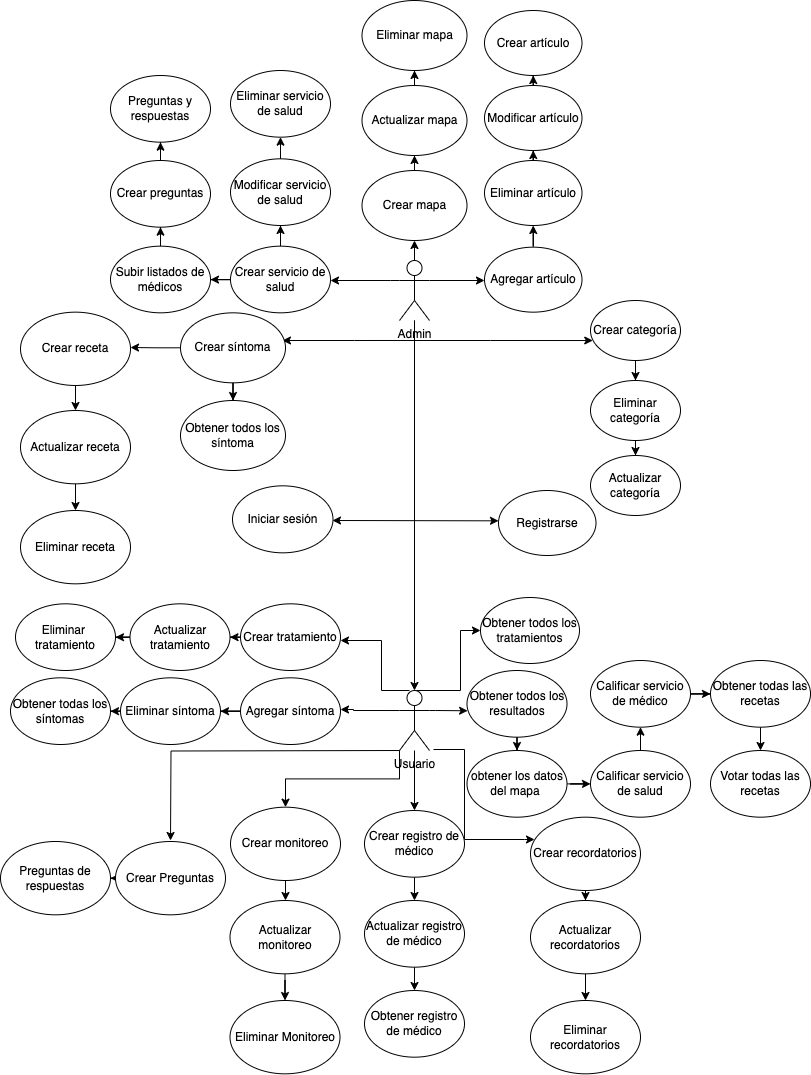
\includegraphics[width=0.7\textwidth]{img/manual/diagrama_casos_de_uso.png}
    \caption{Diagrama de Casos de Uso} \label{Img:Diseno+Casos+de+Uso}
\end{figure} 


% Caso de Uso 1 -> Registro de usuario
\begin{table}[p]
    \centering
    \begin{tabularx}{\linewidth}{ p{0.21\columnwidth} X }
        \toprule
        \textbf{CU-1}    & \textbf{Registro de usuario}\\
        \toprule
        \textbf{Versión}              & 1.0    \\
        \textbf{Autor}                & Roberto Fabián Delgado Pense \\
        \textbf{Requisitos asociados} & RF-1.1 \\ 
        \textbf{Descripción}          & Permite al usuario registrarse en el sistema. \\
        \textbf{Precondición}         & El usuario ha ingresado su dirección de correo electrónico y contraseña. \\
        \textbf{Acciones}             &
        \begin{enumerate}
            \item El sistema verifica las credenciales ingresadas.
            \item Si el correo electrónico y contraseña son válidas, el sistema lo guarda en la base de datos.
            \item El sistema devuelve un mensaje satisfactorio.
        \end{enumerate}\\
        \textbf{Postcondición}        & - \\
        \textbf{Excepciones}          & Si el correo electrónico o la contraseña no cumple los criterios el sistema devuelve un mensaje de error. \\
        \textbf{Importancia}          & Alta \\
        \bottomrule
    \end{tabularx}
    \caption{CU-1 Registro de usuario.}
\end{table}

\begin{table}[p]
    \centering
    \begin{tabularx}{\linewidth}{ p{0.21\columnwidth} X }
        \toprule
        \textbf{CU-2}    & \textbf{Autenticación del usuario}\\
        \toprule
        \textbf{Versión}              & 1.0    \\
        \textbf{Autor}                & Roberto Fabián Delgado Pense \\
        \textbf{Requisitos asociados} & RF-1.2 \\ 
        \textbf{Descripción}          & Permite al usuario ingresar al sistema. \\
        \textbf{Precondición}         & El usuario ha ingresado su dirección de correo electrónico y contraseña. \\
        \textbf{Acciones}             &
        \begin{enumerate}
            \item El sistema verificará las credenciales ingresadas.
            \item Si el correo electrónico y contraseña son válidas, el sistema genera un token JWT válido.
            \item El sistema devuelve el token JWT.
        \end{enumerate}\\
        \textbf{Postcondición}        & El usuario recibe un token JWT válido por 24 horas.\\
        \textbf{Excepciones}          & Si las credenciales ingresadas por el usuario son inválidas, el sistema devuelve una respuesta HTTP con el código 401 (No autorizado) y un mensaje. \\
        \textbf{Importancia}          & Alta \\
        \bottomrule
    \end{tabularx}
    \caption{CU-2 Autenticación del usuario.}
\end{table}

% Caso de Uso 3 -> Actualización de usuario
\begin{table}[p]
	\centering
	\begin{tabularx}{\linewidth}{ p{0.21\columnwidth} p{0.71\columnwidth} }
		\toprule
		\textbf{CU-3}    & \textbf{Actualización del usuario}\\
		\toprule
		\textbf{Versión}              & 1.0    \\
		\textbf{Autor}                & Roberto Fabián Delgado Pense \\
		\textbf{Requisitos asociados} & RF-1.3 \\ 
		\textbf{Descripción}          & Permite al usuario actualizar sus datos. \\
		\textbf{Precondición}         & El usuario se ha autenticado y ha proporcionado información válida para                                             actualizar su perfil. \\
		\textbf{Acciones}             &
		\begin{enumerate}
			\def\labelenumi{\arabic{enumi}.}
			\tightlist
                \item El sistema verifica que el usuario que realiza la solicitud se encuentre autenticado.
			\item El sistema busca al usuario en la base de datos utilizando un identificador único (UUID)                      proporcionado por el token JWT.
                \item El sistema actualiza los datos del usuario en la base de datos.
                \item El sistema devuelve una respuesta de éxito al usuario.
            \end{enumerate}\\
		\textbf{Postcondición}        & Se actualizan los datos del usuario en la base de datos.\\
  		\textbf{Excepciones}          & 
                \begin{enumerate}
			\def\labelenumi{\arabic{enumi}.}
			\tightlist
			\item Si el usuario no se encuentra autenticado el sistema devuelve una respuesta HTTP con el código 401 (No autorizado) y un mensaje.
                \item Si los datos proporcionados por el usuario no son válidos o el usuario no se                           encuentra en la base de datos, el sistema devuelve un mensaje de error. 
            \end{enumerate} \\
		\textbf{Importancia}          & Alta \\
		\bottomrule
	\end{tabularx}
	\caption{CU-3 Actualización del usuario.}
\end{table}

% Caso de Uso 4 -> Obtener información del usuario
\begin{table}[p]
	\centering
	\begin{tabularx}{\linewidth}{ p{0.21\columnwidth} p{0.71\columnwidth} }
		\toprule
		\textbf{CU-4}    & \textbf{Obtener información del usuario}\\
		\toprule
		\textbf{Versión}              & 1.0    \\
		\textbf{Autor}                & Roberto Fabián Delgado Pense \\
		\textbf{Requisitos asociados} & RF-1.4 \\ 
		\textbf{Descripción}          & Permite al usuario obtener su información. \\
		\textbf{Precondición}         & El usuario ha realizado una solicitud para obtener su información personal. \\
		\textbf{Acciones}             &
		\begin{enumerate}
			\def\labelenumi{\arabic{enumi}.}
			\tightlist
			\item El sistema busca al usuario en la base de datos utilizando el identificador único (UUID).
			\item El sistema devuelve la información del usuario que realizó la solicitud.
            \end{enumerate}\\
		\textbf{Postcondición}        & El usuario recibe su propia información personal.\\
		\textbf{Excepciones}          & 
                \begin{enumerate}
			\def\labelenumi{\arabic{enumi}.}
			\tightlist
			\item Si el usuario no se encuentra autenticado el sistema devuelve una respuesta HTTP con el código 401 (No autorizado) y un mensaje.
                \item   Si el usuario no se encuentra en la base de datos, el sistema devuelve un                                            mensaje de error. 
            \end{enumerate}\\
		\textbf{Importancia}          & Alta \\
		\bottomrule
	\end{tabularx}
	\caption{CU-4 Obtener información del usuario.}
\end{table}

% Caso de Uso 5 -> Actualizar el estado de activación del usuario
\begin{table}[p]
	\centering
	\begin{tabularx}{\linewidth}{ p{0.21\columnwidth} p{0.71\columnwidth} }
		\toprule
		\textbf{CU-5}    & \textbf{Actualizar estado de activación del usuario}\\
		\toprule
		\textbf{Versión}              & 1.0    \\
		\textbf{Autor}                & Roberto Fabián Delgado Pense \\
		\textbf{Requisitos asociados} & RF-1.5 \\ 
		\textbf{Descripción}          & Permite al usuario administrador cambiar el estado de un usuario. \\
		\textbf{Precondición}         & Un usuario administrador ha proporcionado un identificador único de usuario y                                              solicita cambiar el estado de activación de un usuario en particular.\\
		\textbf{Acciones}             &
		\begin{enumerate}
			\def\labelenumi{\arabic{enumi}.}
			\tightlist
			\item El sistema busca al usuario en la base de datos utilizando el identificador único (UUID)
                \item El sistema verifica que el usuario que realiza la solicitud se encuentre autenticado y tenga el        permiso de usuario administrador.
			\item El sistema actualiza el estado de activación del usuario en la base de datos, cambiándolo a activo             o inactivo.
                \item El sistema devuelve una respuesta de éxito.
            \end{enumerate}\\
		\textbf{Postcondición}        & Se actualiza el estado de activación del usuario en la base de datos.\\
  
		\textbf{Excepciones}          & 
                \begin{enumerate}
			\def\labelenumi{\arabic{enumi}.}
			\tightlist
			\item Si el usuario no se encuentra autenticado, o no es usuario administrador el sistema devuelve una                 respuesta HTTP con el código 401 (No autorizado) y un mensaje.
                \item   Si el usuario no se encuentra en la base de datos, el sistema devuelve un                                            mensaje de error. 
            \end{enumerate}\\
		\textbf{Importancia}          & Alta \\
		\bottomrule
	\end{tabularx}
	\caption{CU-5 Actualizar estado de activación del usuario.}
\end{table}

% Caso de Uso 6 -> Actualización de estado de baneo de usuario
\begin{table}[p]
	\centering
	\begin{tabularx}{\linewidth}{ p{0.21\columnwidth} p{0.71\columnwidth} }
		\toprule
		\textbf{CU-6}    & \textbf{Actualización del estado de baneo de usuario}\\
		\toprule
		\textbf{Versión}              & 1.0    \\
		\textbf{Autor}                & Roberto Fabián Delgado Pense \\
		\textbf{Requisitos asociados} & RF-1.6 \\ 
		\textbf{Descripción}          & Permite al usuario administrador banear un usuario. \\
		\textbf{Precondición}         & Un usuario administrador ha proporcionado un identificador único de usuario (UUID) y el                                          nuevo estado de baneo para un usuario en particular.\\
		\textbf{Acciones}             &
		\begin{enumerate}
			\def\labelenumi{\arabic{enumi}.}
			\tightlist
                \item El sistema verifica que el usuario que realiza la solicitud se encuentre autenticado y tenga el  permiso de usuario administrador.
			\item El sistema busca al usuario en la base de datos utilizando el identificador único (UUID)
			\item El sistema actualiza el estado de activación del usuario en la base de datos, cambiándolo a activo             o inactivo.
                \item El sistema devuelve una respuesta de éxito.
            \end{enumerate}\\
		\textbf{Postcondición}        & Se actualiza el estado de activación del usuario en la base de datos.\\
		\textbf{Excepciones}          &
              \begin{enumerate}
			\def\labelenumi{\arabic{enumi}.}
			\tightlist
			\item Si el usuario no se encuentra autenticado, o no es usuario administrador, el sistema devuelve una                 respuesta HTTP con el código 401 (No autorizado) y un mensaje.
                \item   Si el usuario no se encuentra en la base de datos, el sistema devuelve un                                            mensaje de error. 
            \end{enumerate}\\
  		\textbf{Importancia}          & Alta \\
		\bottomrule
	\end{tabularx}
	\caption{CU-6 Actualización del estado de baneo de usuario.}
\end{table}

% Caso de Uso 7 -> Crear un artículo
\begin{table}[p]
	\centering
	\begin{tabularx}{\linewidth}{ p{0.21\columnwidth} p{0.71\columnwidth} }
		\toprule
		\textbf{CU-7}    & \textbf{Crear un artículo}\\
		\toprule
		\textbf{Versión}              & 1.0    \\
		\textbf{Autor}                & Roberto Fabián Delgado Pense \\
		\textbf{Requisitos asociados} & RF-2.1, RF-2.2.1, RF-3.2 \\ 
		\textbf{Descripción}          & Permite al usuario administrador crear un artículo. \\
		\textbf{Precondición}         & El usuario administrador ha proporcionado el título, contenido  y imagen para el artículo.\\
		\textbf{Acciones}             &
		\begin{enumerate}
			\def\labelenumi{\arabic{enumi}.}
			\tightlist
			\item El sistema recibe una solicitud HTTP para crear un artículo.
                \item El sistema verifica que el usuario que realiza la solicitud se encuentre autenticado y tenga el permiso de usuario administrador.
			\item El sistema extrae el título, contenido e imagen de la solicitud.
                \item Si la autenticación fue exitosa, el sistema genera un identificador único (UUID) para el artículo.
                \item El sistema guarda el artículo en la base de datos, asociándolo con el identificador del usuario         administrador.
                \item El sistema devuelve una respuesta HTTP con el código 200 (OK) y el artículo creado.            \end{enumerate}\\
		\textbf{Postcondición}        & El artículo fue creado y guardado en la base de datos.\\
		\textbf{Excepciones}          & 
            \begin{enumerate}
			\def\labelenumi{\arabic{enumi}.}
			\tightlist
			\item Si el usuario no se encuentra autenticado, el sistema devuelve una respuesta HTTP con el código            401 (No autorizado).
			\item Si no se proporciona el título, contenido e imagen válida para el artículo, el sistema devuelve una respuesta HTTP con el código 400 (Solicitud incorrecta).
            \end{enumerate}\\
		\textbf{Importancia}          & Alta \\
		\bottomrule
	\end{tabularx}
	\caption{CU-7 Crear un artículo.}
\end{table}

% Caso de Uso 8 -> Obtener todos los artículos
\begin{table}[p]
	\centering
	\begin{tabularx}{\linewidth}{ p{0.21\columnwidth} p{0.71\columnwidth} }
		\toprule
		\textbf{CU-8}    & \textbf{Obtener todos los artículos}\\
		\toprule
		\textbf{Versión}              & 1.0    \\
		\textbf{Autor}                & Roberto Fabián Delgado Pense \\
		\textbf{Requisitos asociados} & RF-2.2 \\ 
		\textbf{Descripción}          & Permite a los usuarios obtener un listado de los                                             artículos. \\
		\textbf{Precondición}         & La base de datos esta disponible. \\
		\textbf{Acciones}             &
		\begin{enumerate}
			\def\labelenumi{\arabic{enumi}.}
			\tightlist
			\item El sistema recibe una solicitud HTTP para obtener todos los artículos.
			\item El sistema verifica que el usuario que realiza la solicitud este autenticado.
                \item Si la autenticación fue exitosa, el sistema recupera todos los artículos guardados en la base        de datos.
                \item El sistema devuelve una respuesta HTTP con el código 200 (OK) y la lista de todos los artículos        recuperados.
            \end{enumerate}\\
		\textbf{Postcondición}        & - \\
		\textbf{Excepciones}          & Si el usuario no se encuentra autenticado, el sistema devuelve una respuesta HTTP con el código            401 (No autorizado) y un mensaje. \\
		\textbf{Importancia}          & Media \\
		\bottomrule
	\end{tabularx}
	\caption{CU-8 Obtener todos los artículos.}
\end{table}

% Caso de Uso 9 -> Actualizar un artículo
\begin{table}[p]
	\centering
	\begin{tabularx}{\linewidth}{ p{0.21\columnwidth} p{0.71\columnwidth} }
		\toprule
		\textbf{CU-9}    & \textbf{Actualizar un artículo}\\
		\toprule
		\textbf{Versión}              & 1.0    \\
		\textbf{Autor}                & Roberto Fabián Delgado Pense \\
		\textbf{Requisitos asociados} & RF-2.3, RF-2.2.1, RF-3.2 \\ 
		\textbf{Descripción}          & Permite al usuario administrador actualizar un artículo. \\
		\textbf{Precondición}         & 
  \begin{enumerate}
			\def\labelenumi{\arabic{enumi}.}
			\tightlist
			\item   El usuario administrador ha proporcionado un identificador único (UUID), de artículo existente.
			\item   El usuario administrador ha proporcionado los datos que necesita actualizar en el artículo, incluyendo el título, contenido e imagen.
            \end{enumerate}\\
		\textbf{Acciones}             &
		\begin{enumerate}
			\def\labelenumi{\arabic{enumi}.}
			\tightlist
			\item El sistema recibe una solicitud HTTP para actualizar un artículo.
                \item El sistema verifica que el usuario que realiza la solicitud se encuentre autenticado y tenga el        permiso de usuario administrador.
			\item El sistema extrae el identificador único (UUID) del artículo desde la URL de la solicitud.
                \item Si la autenticación fue exitosa, el sistema busca en la base de datos el artículo usando el identificador único (UUID).
                \item El sistema actualiza el título, contenido e imagen del artículo con los datos proporcionados.
                \item El sistema devuelve una respuesta HTTP con el código 200 (OK) y el artículo actualizado.
            \end{enumerate}\\
		\textbf{Postcondición}        & El artículo fue actualizado en la base de datos con los nuevos datos                                           proporcionados. \\
		\textbf{Excepciones}          & 
            \begin{enumerate}
			\def\labelenumi{\arabic{enumi}.}
			\tightlist
   			\item Si el usuario no se encuentra autenticado, o no es usuario administrador, el sistema devuelve una                 respuesta HTTP con el código 401 (No autorizado) y un mensaje.
                \item Si no se proporciona un identificador único (UUID) válido de un artículo, el sistema devuelve una respuesta HTTP con el código 400 (Solicitud incorrecta).
                \item Si no se proporcionan datos correctos para el título, contenido e imagen para el artículo, el sistema devuelve una respuesta HTTP con el código 400 (Solicitud incorrecta).
            \end{enumerate}\\
		\textbf{Importancia}          & Alta \\
		\bottomrule
	\end{tabularx}
	\caption{CU-9 Actualizar un artículo.}
\end{table}

% Caso de Uso 10 -> Eliminar un artículo
\begin{table}[p]
	\centering
	\begin{tabularx}{\linewidth}{ p{0.21\columnwidth} p{0.71\columnwidth} }
		\toprule
		\textbf{CU-10}    & \textbf{Eliminar un artículo}\\
		\toprule
		\textbf{Versión}              & 1.0    \\
		\textbf{Autor}                & Roberto Fabián Delgado Pense \\
		\textbf{Requisitos asociados} & RF-2.4 \\ 
		\textbf{Descripción}          & Permite al usuario administrador eliminar un artículo. \\
		\textbf{Precondición}         & El usuario administrador ha proporcionado un identificador único (UUID) de artículo existente.\\
		\textbf{Acciones}             &
		\begin{enumerate}
			\def\labelenumi{\arabic{enumi}.}
			\tightlist
			\item El sistema recibe una solicitud HTTP para eliminar un artículo.
                   \item El sistema verifica que el usuario que realiza la solicitud se encuentre autenticado y tenga el  permiso de usuario administrador.
			\item El sistema extrae el identificador único (UUID) del artículo desde la URL de la solicitud.
                \item Si la autenticación fue exitosa, el sistema busca en la base de datos el artículo usando el identificador único (UUID).
                \item El sistema elimina el artículo de la base de datos.
                \item El sistema devuelve una respuesta HTTP con el código 200 (OK) y un mensaje.
            \end{enumerate}\\
		\textbf{Postcondición}        & El artículo fue eliminado de la base de datos.\\
		\textbf{Excepciones}          & 
            \begin{enumerate}
			\def\labelenumi{\arabic{enumi}.}
			\tightlist
   			\item Si el usuario no se encuentra autenticado, o no es usuario administrador, el sistema devuelve una                 respuesta HTTP con el código 401 (No autorizado) y un mensaje.
                \item Si no se proporciona un identificador único (UUID) válido de un artículo, el sistema devuelve una respuesta HTTP con el código 400 (Solicitud incorrecta).
            \end{enumerate}\\
		\textbf{Importancia}          & Alta \\
		\bottomrule
	\end{tabularx}
	\caption{CU-10 Eliminar un artículo.}
\end{table}

% Caso de Uso 11 -> Agregar categoría a un artículo
\begin{table}[p]
	\centering
	\begin{tabularx}{\linewidth}{ p{0.21\columnwidth} p{0.71\columnwidth} }
		\toprule
		\textbf{CU-11}    & \textbf{Agregar categoría a un artículo}\\
		\toprule
		\textbf{Versión}              & 1.0    \\
		\textbf{Autor}                & Roberto Fabián Delgado Pense \\
		\textbf{Requisitos asociados} & RF-xx, RF-xx \\ 
		\textbf{Descripción}          & Permite al usuario administrador agregar una categoría a un artículo. \\
		\textbf{Precondición}         & 
  		\begin{enumerate}
			\def\labelenumi{\arabic{enumi}.}
			\tightlist
			\item El usuario administrador ha proporcionado un identificador único (UUID) de artículo existente.
			\item El usuario administrador ha proporcionado un identificador único (UUID) de categoría existente.
            \end{enumerate}\\
		\textbf{Acciones}             &
		\begin{enumerate}
			\def\labelenumi{\arabic{enumi}.}
			\tightlist
			\item El sistema recibe una solicitud HTTP para agregar una categoría a un artículo.
                \item El sistema verifica que el usuario administrador que realiza la solicitud se encuentre autenticado y tenga el permiso de administrador.
			\item El sistema extrae los identificadores únicos (UUID) del artículo y la categoría desde la                  solicitud.
                \item Si la autenticación fue exitosa, el sistema busca en la base de datos el artículo y la categoría usando los identificadores únicos (UUID).
                \item El sistema asocia el artículo con la categoría en la base de datos.
                \item El sistema devuelve una respuesta HTTP con el código 200 (OK).
            \end{enumerate}\\
		\textbf{Postcondición}        & El artículo fue asociado a la categoría en la base de datos.\\
		\textbf{Excepciones}          & 
            \begin{enumerate}
			\def\labelenumi{\arabic{enumi}.}
			\tightlist
   			\item Si el usuario no se encuentra autenticado, o no es usuario administrador, el sistema devuelve una                 respuesta HTTP con el código 401 (No autorizado) y un mensaje.
                \item Si no se proporciona un identificador único (UUID) válido de un artículo, el sistema devuelve una respuesta HTTP con el código 400 (Solicitud incorrecta).
            \end{enumerate}\\
		\textbf{Importancia}          & Media \\
		\bottomrule
	\end{tabularx}
	\caption{CU-11 Agregar categoría a un artículo.}
\end{table}

% Caso de Uso 12 -> Eliminar categoría de un artículo
\begin{table}[p]
	\centering
	\begin{tabularx}{\linewidth}{ p{0.21\columnwidth} p{0.71\columnwidth} }
		\toprule
		\textbf{CU-12}    & \textbf{Eliminar categoría a un artículo}\\
		\toprule
		\textbf{Versión}              & 1.0    \\
		\textbf{Autor}                & Roberto Fabián Delgado Pense \\
		\textbf{Requisitos asociados} & RF-2.1, RF-3.1, RF-3.4 \\ 
		\textbf{Descripción}          & Permite al usuario administrador eliminar la categoría de un artículo. \\
		\textbf{Precondición}         & El usuario administrador ha proporcionado un identificador único (UUID) de artículo existente. \\
		\textbf{Acciones}             &
		\begin{enumerate}
			\def\labelenumi{\arabic{enumi}.}
			\tightlist
			\item El sistema recibe una solicitud HTTP para agregar una categoría a un artículo.
                \item El sistema verifica que el usuario que realiza la solicitud se encuentre autenticado y tenga el permiso de usuario administrador.
			\item El sistema extrae los identificadores únicos (UUID) del artículo y la categoría desde la                  solicitud.
                \item Si la autenticación fue exitosa, el sistema busca en la base de datos el artículo y la categoría usando los identificadores únicos (UUID).
                \item El sistema asocia el artículo con la categoría en la base de datos.
                \item El sistema devuelve una respuesta HTTP con el código 200 (OK).
            \end{enumerate}\\
		\textbf{Postcondición}        & El artículo fue disociado de la categoría en la base de datos.\\
		\textbf{Excepciones}          & 
            \begin{enumerate}
			\def\labelenumi{\arabic{enumi}.}
			\tightlist
   			\item Si el usuario no se encuentra autenticado, o no es administrador, el sistema devuelve una                 respuesta HTTP con el código 401 (No autorizado) y un mensaje.
                \item Si no se proporciona un identificador único (UUID) válido de un artículo, el sistema devuelve una respuesta HTTP con el código 400 (Solicitud incorrecta).
            \end{enumerate}\\
		\textbf{Importancia}          & Media \\
		\bottomrule
	\end{tabularx}
	\caption{CU-12 Eliminar categoría a un artículo.}
\end{table}

% Caso de Uso 13 -> Crear categoría
\begin{table}[p]
	\centering
	\begin{tabularx}{\linewidth}{ p{0.21\columnwidth} p{0.71\columnwidth} }
		\toprule
		\textbf{CU-13}    & \textbf{Crear categoría}\\
		\toprule
		\textbf{Versión}              & 1.0    \\
		\textbf{Autor}                & Roberto Fabián Delgado Pense \\
		\textbf{Requisitos asociados} & RF-3.1 \\ 
		\textbf{Descripción}          & Permite al usuario administrador crear una categoría. \\
		\textbf{Precondición}         & El usuario tiene permisos de administrador. \\
		\textbf{Acciones}             &
		\begin{enumerate}
			\def\labelenumi{\arabic{enumi}.}
			\tightlist
			\item El sistema recibe una solicitud HTTP para crear una nueva categoría.
                \item El sistema verifica que el usuario que realiza la solicitud se encuentre autenticado y tenga el permiso de usuario administrador.
			\item El sistema valida la solicitud y verifica que los datos para crear la categoría sean correctos.
                \item El sistema crea la categoría en la base de datos.
                \item El sistema devuelve una respuesta HTTP con el código 200 (OK).
            \end{enumerate}\\
		\textbf{Postcondición}        & La categoría fue creada en la base de datos.\\
		\textbf{Excepciones}          & 
            \begin{enumerate}
			\def\labelenumi{\arabic{enumi}.}
			\tightlist
   			\item Si el usuario no se encuentra autenticado, o no es usuario administrador, el sistema devuelve una                 respuesta HTTP con el código 401 (No autorizado) y un mensaje.
            \end{enumerate}\\
		\textbf{Importancia}          & Alta \\
		\bottomrule
	\end{tabularx}
	\caption{CU-13 Crear categoría.}
\end{table}

% Caso de Uso 14 -> Obtener todas las categorías
\begin{table}[p]
	\centering
	\begin{tabularx}{\linewidth}{ p{0.21\columnwidth} p{0.71\columnwidth} }
		\toprule
		\textbf{CU-14}    & \textbf{Obtener todas las categorías}\\
		\toprule
		\textbf{Versión}              & 1.0    \\
		\textbf{Autor}                & Roberto Fabián Delgado Pense \\
		\textbf{Requisitos asociados} & RF-3.2 \\ 
		\textbf{Descripción}          & Permite al usuario administrador obtener todas las categorías. \\
		\textbf{Precondición}         & El usuario tiene permisos de administrador. \\
		\textbf{Acciones}             &
		\begin{enumerate}
			\def\labelenumi{\arabic{enumi}.}
			\tightlist
			\item El sistema recibe una solicitud HTTP para obtener las categorías.
                \item El sistema verifica que el usuario que realiza la solicitud se encuentre autenticado y tenga el permiso de usuario administrador.
			\item El sistema obtiene todas las categorías guardadas en la base de datos.
                \item El sistema devuelve una respuesta HTTP con el código 200 (OK).
            \end{enumerate}\\
		\textbf{Postcondición}        & La categoría fue creada en la base de datos.\\
		\textbf{Excepciones}          & 
            \begin{enumerate}
			\def\labelenumi{\arabic{enumi}.}
			\tightlist
   			\item Si el usuario no se encuentra autenticado, o no es usuario administrador, el sistema devuelve una                 respuesta HTTP con el código 401 (No autorizado) y un mensaje.
                \item Si ocurre un error al obtener las categorías, el sistema devuelve una respuesta con el código de estado 500 Internal Server Error y un mensaje.
            \end{enumerate}\\
		\textbf{Importancia}          & Media \\
		\bottomrule
	\end{tabularx}
	\caption{CU-14 Obtener todas las categorías.}
\end{table}

% Caso de Uso 15 -> Actualizar una categoría
\begin{table}[p]
	\centering
	\begin{tabularx}{\linewidth}{ p{0.21\columnwidth} p{0.71\columnwidth} }
		\toprule
		\textbf{CU-15}    & \textbf{Actualizar una categoría}\\
		\toprule
		\textbf{Versión}              & 1.0    \\
		\textbf{Autor}                & Roberto Fabián Delgado Pense \\
		\textbf{Requisitos asociados} & RF-3.3 \\ 
		\textbf{Descripción}          & Permite al usuario administrador actualizar una categoría. \\
		\textbf{Precondición}         & El usuario tiene permisos de administrador. \\
		\textbf{Acciones}             &
		\begin{enumerate}
			\def\labelenumi{\arabic{enumi}.}
			\tightlist
                \item El sistema verifica que el usuario que realiza la solicitud se encuentre autenticado y tenga el permiso de usuario administrador.
			\item El usuario ha proporcionado un identificador único (UUID), de categoría existente.
			\item El sistema valida la existencia de la categoría en la base de datos.
                \item El sistema actualiza los datos de la categoría con los nuevos valores proporcionados en la solicitud.
                \item El sistema devuelve una respuesta HTTP con el código 200 (OK).
            \end{enumerate}\\
		\textbf{Postcondición}        & La categoría se actualiza correctamente en la base de datos.\\
		\textbf{Excepciones}          & 
            \begin{enumerate}
			\def\labelenumi{\arabic{enumi}.}
			\tightlist
   			\item Si el usuario no se encuentra autenticado, o no es usuario administrador, el sistema devuelve una                 respuesta HTTP con el código 401 (No autorizado) y un mensaje.
                \item   Si la categoría no se encuentra en la base de datos, el sistema devuelve un                           una respuesta HTTP con el código 404 (No encontrado) y un mensaje. 
                \item Si ocurre un error al actualizar la categoría, el sistema devuelve una respuesta con el código de estado 500 (Error interno del servidor) y un mensaje
            \end{enumerate}\\
		\textbf{Importancia}          & Alta \\
		\bottomrule
	\end{tabularx}
	\caption{CU-15 Actualizar una categoría.}
\end{table}

% Caso de Uso 16 -> Eliminar una categoría
\begin{table}[p]
	\centering
	\begin{tabularx}{\linewidth}{ p{0.21\columnwidth} p{0.71\columnwidth} }
		\toprule
		\textbf{CU-16}    & \textbf{Eliminar una categoría}\\
		\toprule
		\textbf{Versión}              & 1.0    \\
		\textbf{Autor}                & Roberto Fabián Delgado Pense \\
		\textbf{Requisitos asociados} & RF-3.4 \\ 
		\textbf{Descripción}          & Permite al usuario administrador eliminar una categoría. \\
		\textbf{Precondición}         & El usuario ha proporcionado un identificador único (UUID) de categoría existente.\\
		\textbf{Acciones}             &
		\begin{enumerate}
			\def\labelenumi{\arabic{enumi}.}
			\tightlist
			\item El sistema recibe una solicitud HTTP para eliminar una categoría.
                   \item El sistema verifica que el usuario que realizar la solicitud se encuentre autenticado y tenga el permiso de usuario administrador.
			\item El sistema extrae el identificador único (UUID) de la categoría desde la URL de la solicitud.
                \item Si la autenticación fue exitosa, el sistema busca en la base de datos la categoría usando el identificador único (UUID).
                \item El sistema elimina la categoría de la base de datos.
                \item El sistema devuelve una respuesta HTTP con el código 200 (OK) y la categoría fue eliminada.
            \end{enumerate}\\
		\textbf{Postcondición}        & La categoría fue eliminada de la base de datos.\\
		\textbf{Excepciones}          & 
            \begin{enumerate}
			\def\labelenumi{\arabic{enumi}.}
			\tightlist
   			\item Si el usuario no se encuentra autenticado, o no es usuario administrador, el sistema devuelve una                 respuesta HTTP con el código 401 (No autorizado) y un mensaje.
                \item   Si la categoría no se encuentra en la base de datos, el sistema devuelve un                           una respuesta HTTP con el código 404 (No encontrado) y un mensaje. 
                \item Si ocurre un error al eliminar la categoría, el sistema devuelve una respuesta con el código de estado 500 (Error interno del servidor) y un mensaje
            \end{enumerate}\\
		\textbf{Importancia}          & Alta \\
		\bottomrule
	\end{tabularx}
	\caption{CU-16 Eliminar una categoría.}
\end{table}

% Caso de Uso 17 -> Crear pregunta
\begin{table}[p]
	\centering
	\begin{tabularx}{\linewidth}{ p{0.21\columnwidth} p{0.71\columnwidth} }
		\toprule
		\textbf{CU-17}    & \textbf{Crear pregunta}\\
		\toprule
		\textbf{Versión}              & 1.0    \\
		\textbf{Autor}                & Roberto Fabián Delgado Pense \\
		\textbf{Requisitos asociados} & RF-4.1 \\ 
		\textbf{Descripción}          & Permite a los usuarios crear preguntas. \\
		\textbf{Precondición}         & El usuario debe estar autenticado.\\
		\textbf{Acciones}             &
		\begin{enumerate}
			\def\labelenumi{\arabic{enumi}.}
			\tightlist
			\item El sistema recibe una solicitud HTTP para crear una pregunta.
                \item El sistema verifica que el usuario que realiza la solicitud este autenticado.
			\item El sistema valida la solicitud y extrae el texto de la pregunta.
                \item El sistema crea una nueva pregunta en la base de datos, asociándola al usuario actual.
                \item El sistema devuelve una respuesta HTTP con el código 200 (OK) y la pregunta creada.            \end{enumerate}\\
		\textbf{Postcondición}        & La pregunta fue creada y guardada en la base de datos.\\
		\textbf{Excepciones}          & 
            \begin{enumerate}
			\def\labelenumi{\arabic{enumi}.}
			\tightlist
			\item Si el usuario no se encuentra autenticado, el sistema devuelve una respuesta HTTP con el código            401 (No autorizado).
			\item Si la solicitud es inválida o los datos de la pregunta son incorrectos para la pregunta, el sistema devuelve una respuesta HTTP con el código 400 (Solicitud incorrecta) y un mensaje de error.
            \end{enumerate}\\
		\textbf{Importancia}          & Alta \\
		\bottomrule
	\end{tabularx}
	\caption{CU-17 Crear pregunta.}
\end{table}

% Caso de Uso 18 -> Obtener todas las preguntas
\begin{table}[p]
	\centering
	\begin{tabularx}{\linewidth}{ p{0.21\columnwidth} p{0.71\columnwidth} }
		\toprule
		\textbf{CU-18}    & \textbf{Obtener todas las preguntas}\\
		\toprule
		\textbf{Versión}              & 1.0    \\
		\textbf{Autor}                & Roberto Fabián Delgado Pense \\
		\textbf{Requisitos asociados} & RF-4.2 \\ 
		\textbf{Descripción}          & Permite a los usuarios obtener todas las  preguntas. \\
		\textbf{Precondición}         & El usuario debe estar autenticado.\\
		\textbf{Acciones}             &
		\begin{enumerate}
			\def\labelenumi{\arabic{enumi}.}
			\tightlist
			\item El sistema recibe una solicitud HTTP para obtener las preguntas.
                \item El sistema verifica que el usuario que realiza la solicitud se encuentre autenticado.
			\item El sistema obtiene todas las preguntas guardadas en la base de datos.
                \item El sistema devuelve una respuesta HTTP con el código 200 (OK).          
            \end{enumerate}\\
		\textbf{Postcondición}        & - \\
		\textbf{Excepciones}          & Si el usuario no se encuentra autenticado, el sistema devuelve una respuesta HTTP con el código 401 (No autorizado). \\
		\textbf{Importancia}          & Media \\
		\bottomrule
	\end{tabularx}
	\caption{CU-18 Obtener todas las preguntas.}
\end{table}

% Caso de Uso 19 -> Crear respuesta a pregunta
\begin{table}[p]
	\centering
	\begin{tabularx}{\linewidth}{ p{0.21\columnwidth} p{0.71\columnwidth} }
		\toprule
		\textbf{CU-19}    & \textbf{Crear respuesta a pregunta}\\
		\toprule
		\textbf{Versión}              & 1.0    \\
		\textbf{Autor}                & Roberto Fabián Delgado Pense \\
		\textbf{Requisitos asociados} & RF-4.3 \\ 
		\textbf{Descripción}          & Permite a los usuarios crear respuesta a una pregunta.\\
		\textbf{Precondición}         & 
  		\begin{enumerate}
			\def\labelenumi{\arabic{enumi}.}
			\tightlist
                \item El usuario debe estar autenticado.
                \item La pregunta a la que va a responder existe en el sistema.
                \end{enumerate}\\
            \textbf{Acciones}             &
		\begin{enumerate}
			\def\labelenumi{\arabic{enumi}.}
			\tightlist
			\item El sistema recibe una solicitud HTTP para crear una respuesta a una pregunta.
                \item El sistema verifica que el usuario que realiza la solicitud este autenticado.
			\item El sistema extrae el identificador único (UUID) de la pregunta desde la URL de la solicitud.
			\item El sistema valida la solicitud y extrae el texto de la respuesta.
                \item El sistema crea una nueva respuesta a la pregunta en la base de datos, asociándola al usuario actual.
                \item El sistema devuelve una respuesta HTTP con el código 200 (OK) y la respuesta creada.            \end{enumerate}\\
		\textbf{Postcondición}        & La respuesta fue creada y guardada en la base de datos.\\
		\textbf{Excepciones}          & 
            \begin{enumerate}
			\def\labelenumi{\arabic{enumi}.}
			\tightlist
			\item Si el usuario no se encuentra autenticado, el sistema devuelve una respuesta HTTP con el código            401 (No autorizado).
			\item Si la solicitud es inválida o los datos de la respuesta son incorrectos para la pregunta, el sistema devuelve una respuesta HTTP con el código 400 (Solicitud incorrecta) y un mensaje de error.
            \end{enumerate}\\
		\textbf{Importancia}          & Alta \\
		\bottomrule
	\end{tabularx}
	\caption{CU-19 Crear respuesta a pregunta.}
\end{table}

% Caso de Uso 20 -> Obtener todas las respuestas de una pregunta
\begin{table}[p]
	\centering
	\begin{tabularx}{\linewidth}{ p{0.21\columnwidth} p{0.71\columnwidth} }
		\toprule
		\textbf{CU-20}    & \textbf{Obtener todas las respuestas de una pregunta}\\
		\toprule
		\textbf{Versión}              & 1.0    \\
		\textbf{Autor}                & Roberto Fabián Delgado Pense \\
		\textbf{Requisitos asociados} & RF-4.4 \\ 
		\textbf{Descripción}          & Permite a los usuarios obtener todas las  respuestas a una pregunta. \\
		\textbf{Precondición}         & 
  		\begin{enumerate}
			\def\labelenumi{\arabic{enumi}.}
			\tightlist
			\item El usuario debe estar autenticado en el sistema.
                \item La pregunta debe existir en el sistema.        
            \end{enumerate}\\
            
		\textbf{Acciones}             &
		\begin{enumerate}
			\def\labelenumi{\arabic{enumi}.}
			\tightlist
			\item El sistema recibe una solicitud HTTP para obtener todas las respuestas de una pregunta         
                        específica.
                \item El sistema verifica que el usuario que realiza la solicitud se encuentre autenticado.
			\item El sistema obtiene todas las respuestas relacionada a una pregunta guardada en la base de datos.
                \item El sistema devuelve una respuesta HTTP con el código 200 (OK).          
            \end{enumerate}\\
		\textbf{Postcondición}        & - \\
		\textbf{Excepciones}          & 
              \begin{enumerate}
			\def\labelenumi{\arabic{enumi}.}
			\tightlist
			\item   Si el usuario no se encuentra autenticado, el sistema devuelve una respuesta HTTP con el código 401 (No autorizado).
			\item Si no existen respuestas para la pregunta se retorna un array vacío.
            \end{enumerate}\\
		\textbf{Importancia}          & Media \\
		\bottomrule
	\end{tabularx}
	\caption{CU-20 Obtener todas las respuestas de una pregunta.}
\end{table}

% Caso de Uso 21 -> Crear receta
\begin{table}[p]
	\centering
	\begin{tabularx}{\linewidth}{ p{0.21\columnwidth} p{0.71\columnwidth} }
		\toprule
		\textbf{CU-21}    & \textbf{Crear receta}\\
		\toprule
		\textbf{Versión}              & 1.0    \\
		\textbf{Autor}                & Roberto Fabián Delgado Pense \\
		\textbf{Requisitos asociados} & RF-5.1 \\ 
		\textbf{Descripción}          & Permite a los usuarios administradores crear recetas. \\
		\textbf{Precondición}         & El usuario tiene permiso de usuario administrador. \\  
		\textbf{Acciones}             &
		\begin{enumerate}
			\def\labelenumi{\arabic{enumi}.}
			\tightlist
			\item El sistema recibe una solicitud HTTP para crear una receta.
                \item El sistema verifica que el usuario que realiza la solicitud se encuentre autenticado y tenga el permiso de usuario administrador.
                \item El sistema valida la solicitud y extrae el nombre, ingredientes, elaboración, tiempo,     imagenes y categoría.
                \item El sistema crea la receta en la base de datos.
                \item El sistema devuelve una respuesta HTTP con el código 200 (OK) y los datos insertados.         
            \end{enumerate}\\
		\textbf{Postcondición}        & La receta fue creada en la base de datos. \\
		\textbf{Excepciones}          & 
              \begin{enumerate}
			\def\labelenumi{\arabic{enumi}.}
			\tightlist
   			\item Si el usuario no se encuentra autenticado, o no es usuario administrador, el sistema devuelve una                 respuesta HTTP con el código 401 (No autorizado) y un mensaje.
                \item   Si la receta no pudo ser creada en la base de datos, el sistema devuelve un                           una respuesta HTTP con el código 500 (Error interno del servidor) y un mensaje. 
            \end{enumerate}\\
		\textbf{Importancia}          & Alta \\
		\bottomrule
	\end{tabularx}
	\caption{CU-21 Crear receta.}
\end{table}

% Caso de Uso 22 -> Obtener todas las recetas
\begin{table}[p]
	\centering
	\begin{tabularx}{\linewidth}{ p{0.21\columnwidth} p{0.71\columnwidth} }
		\toprule
		\textbf{CU-22}    & \textbf{Obtener todas las recetas}\\
		\toprule
		\textbf{Versión}              & 1.0    \\
		\textbf{Autor}                & Roberto Fabián Delgado Pense \\
		\textbf{Requisitos asociados} & RF-5.2 \\ 
		\textbf{Descripción}          & Permite a los usuarios obtener todas las recetas. \\
		\textbf{Precondición}         & El usuario se encuentra autenticado. \\  
		\textbf{Acciones}             &
		\begin{enumerate}
			\def\labelenumi{\arabic{enumi}.}
			\tightlist
			\item El sistema recibe una solicitud HTTP para obtener las recetas.
                \item El sistema verifica que el usuario que realiza la solicitud se encuentre autenticado.
			\item El sistema obtiene todas las recetas guardadas en la base de datos.
                \item El sistema devuelve una respuesta HTTP con el código 200 (OK) y las recetas.         
            \end{enumerate}\\
		\textbf{Postcondición}        & -  \\
		\textbf{Excepciones}          &  Si el usuario no se encuentra autenticado, o no es administrador, el 
                    sistema devuelve una respuesta HTTP con el código 401 (No autorizado) y un mensaje.\\
		\textbf{Importancia}          & Media \\
		\bottomrule
	\end{tabularx}
	\caption{CU-22 Obtener todas las recetas.}
\end{table}

% Caso de Uso 23 -> Actualizar una receta
\begin{table}[p]
	\centering
	\begin{tabularx}{\linewidth}{ p{0.21\columnwidth} p{0.71\columnwidth} }
		\toprule
		\textbf{CU-23}    & \textbf{Actualizar una receta}\\
		\toprule
		\textbf{Versión}              & 1.0    \\
		\textbf{Autor}                & Roberto Fabián Delgado Pense \\
		\textbf{Requisitos asociados} & RF-5.3 \\ 
		\textbf{Descripción}          & Permite al usuario administrador actualizar una receta. \\
		\textbf{Precondición}         & El usuario tiene permisos de usuario administrador. \\
		\textbf{Acciones}             &
		\begin{enumerate}
			\def\labelenumi{\arabic{enumi}.}
			\tightlist
                \item El sistema verifica que el usuario que realiza la solicitud se encuentre autenticado y tenga el permiso de usuario administrador.
			\item El usuario ha proporcionado un identificador único (UUID), de receta existente.
			\item El sistema valida la existencia de la receta en la base de datos.
                \item El extrae el nombre, ingredientes, elaboración, tiempo, imagenes y categoría.
                \item El sistema actualiza los datos de la receta con los nuevos valores proporcionados en la solicitud.
                \item El sistema devuelve una respuesta HTTP con el código 200 (OK) y un mensaje.
            \end{enumerate}\\
		\textbf{Postcondición}        & La receta se actualiza correctamente en la base de datos.\\
		\textbf{Excepciones}          & 
            \begin{enumerate}
			\def\labelenumi{\arabic{enumi}.}
			\tightlist
   			\item Si el usuario no se encuentra autenticado, o no es usuario administrador, el sistema devuelve una                 respuesta HTTP con el código 401 (No autorizado) y un mensaje.
                \item   Si la receta no se encuentra en la base de datos, el sistema devuelve un                           una respuesta HTTP con el código 404 (No encontrado) y un mensaje. 
                \item Si ocurre un error al actualizar la categoría, el sistema devuelve una respuesta con el código de estado 500 (Error interno del servidor) y un mensaje
            \end{enumerate}\\
		\textbf{Importancia}          & Alta \\
		\bottomrule
	\end{tabularx}
	\caption{CU-23 Actualizar una receta.}
\end{table}

% Caso de Uso 24 -> Eliminar una receta
\begin{table}[p]
	\centering
	\begin{tabularx}{\linewidth}{ p{0.21\columnwidth} p{0.71\columnwidth} }
		\toprule
		\textbf{CU-24}    & \textbf{Eliminar una receta}\\
		\toprule
		\textbf{Versión}              & 1.0    \\
		\textbf{Autor}                & Roberto Fabián Delgado Pense \\
		\textbf{Requisitos asociados} & RF-5.4 \\ 
		\textbf{Descripción}          & Permite al usuario administrador eliminar una receta. \\
		\textbf{Precondición}         & El usuario administrador ha proporcionado un identificador único (UUID) de receta existente.\\
		\textbf{Acciones}             &
		\begin{enumerate}
			\def\labelenumi{\arabic{enumi}.}
			\tightlist
			\item El sistema recibe una solicitud HTTP para eliminar una receta.
                   \item El sistema verifica que el usuario que realiza la solicitud se encuentre autenticado y tenga el permiso de usuario administrador.
			\item El sistema extrae el identificador único (UUID) de la receta desde la URL de la solicitud.
                \item El sistema busca en la base de datos la receta usando el identificador único (UUID).
                \item El sistema elimina la receta de la base de datos.
                \item El sistema devuelve una respuesta HTTP con el código 200 (OK) y un mensaje.
            \end{enumerate}\\
		\textbf{Postcondición}        & La receta fue eliminada de la base de datos.\\
		\textbf{Excepciones}          & 
            \begin{enumerate}
			\def\labelenumi{\arabic{enumi}.}
			\tightlist
   			\item Si el usuario no se encuentra autenticado, o no es usuario administrador, el sistema devuelve una                 respuesta HTTP con el código 401 (No autorizado) y un mensaje.
                \item   Si la receta no se encuentra en la base de datos, el sistema devuelve un                           una respuesta HTTP con el código 404 (No encontrado) y un mensaje. 
                \item Si ocurre un error al eliminar la categoría, el sistema devuelve una respuesta con el código de estado 500 (Error interno del servidor) y un mensaje.
            \end{enumerate}\\
		\textbf{Importancia}          & Alta \\
		\bottomrule
	\end{tabularx}
	\caption{CU-24 Eliminar una receta.}
\end{table}

% Caso de Uso 25 -> Votar una receta
\begin{table}[p]
	\centering
	\begin{tabularx}{\linewidth}{ p{0.21\columnwidth} p{0.71\columnwidth} }
		\toprule
		\textbf{CU-25}    & \textbf{Votar una receta}\\
		\toprule
		\textbf{Versión}              & 1.0    \\
		\textbf{Autor}                & Roberto Fabián Delgado Pense \\
		\textbf{Requisitos asociados} & RF-5.5 \\ 
		\textbf{Descripción}          & Permite al usuario votar una receta. \\
		\textbf{Precondición}         & 
  		\begin{enumerate}
			\def\labelenumi{\arabic{enumi}.}
			\tightlist
			\item El usuario se encuentra autenticado.
                \item La receta a votar existe en el sistema.
            \end{enumerate}\\
		\textbf{Acciones}             &
		\begin{enumerate}
			\def\labelenumi{\arabic{enumi}.}
			\tightlist
			\item El sistema recibe una solicitud HTTP para votar una receta.
                \item El sistema verifica que el usuario que realiza la solicitud se encuentre autenticado.
			\item El sistema extrae el identificador único (UUID) de la receta desde la URL y el valor del voto              desde la solicitud.
         	\item El sistema valida que el voto se encuentra entre los valores 1 y 5.
                \item Si el usuario ya ha votado la receta, actualiza la base de datos con el nuevo valor.
                \item Si el usuario no ha votado antes la receta, crea un nuevo registro de voto.
                \item El sistema devuelve una respuesta HTTP con el código 200 (OK) y un mensaje.
            \end{enumerate}\\
		\textbf{Postcondición}        & El voto de la receta se registra exitosamente.\\
		\textbf{Excepciones}          & 
            \begin{enumerate}
			\def\labelenumi{\arabic{enumi}.}
			\tightlist
   			\item Si el usuario no se encuentra autenticado, o no es usuario administrador, el sistema devuelve una                 respuesta HTTP con el código 401 (No autorizado) y un mensaje.
                \item   Si la receta no se encuentra en la base de datos, el sistema devuelve un                           una respuesta HTTP con el código 404 (No encontrado) y un mensaje. 
                \item   Si el valor del voto no se encuentra entre 1 y 5 retorna una error 400 (Solicitud Incorrecta) y un mensaje. 
                \item Si ocurre un error al registrar el voto, el sistema devuelve una respuesta con el código de estado 500 (Error interno del servidor) y un mensaje
            \end{enumerate}\\
		\textbf{Importancia}          & Alta \\
		\bottomrule
	\end{tabularx}
	\caption{CU-25 Votar una receta.}
\end{table}

% Caso de Uso 26 -> Crear médicos
\begin{table}[p]
	\centering
	\begin{tabularx}{\linewidth}{ p{0.21\columnwidth} p{0.71\columnwidth} }
		\toprule
		\textbf{CU-26}    & \textbf{Crear médicos}\\
		\toprule
		\textbf{Versión}              & 1.0    \\
		\textbf{Autor}                & Roberto Fabián Delgado Pense \\
		\textbf{Requisitos asociados} & RF-6.1 \\ 
		\textbf{Descripción}          & Permite a los usuarios administradores crear médicos. \\
		\textbf{Precondición}         & El usuario tiene permiso de usuario administrador. \\  
		\textbf{Acciones}             &
		\begin{enumerate}
			\def\labelenumi{\arabic{enumi}.}
			\tightlist
			\item El sistema recibe una solicitud HTTP para procesar un archivo CSV.
                \item El sistema verifica que el usuario que realiza la solicitud se encuentre autenticado y tenga el permiso de usuario administrador.
                \item El sistema obtiene el archivo CSV de la solicitud.
                \item El sistema lee y decodifica el archivo CSV.
                \item El sistema procesa los registros del archivo CSV y los guarda en la base de datos.
                \item El sistema devuelve una respuesta HTTP con el código 200 (OK) y un mensaje.         
            \end{enumerate}\\
		\textbf{Postcondición}        & El registro de los médicos fue creado en la base de datos. \\
		\textbf{Excepciones}          & 
              \begin{enumerate}
			\def\labelenumi{\arabic{enumi}.}
			\tightlist
   			\item Si el usuario no se encuentra autenticado, o no es usuario administrador, el sistema devuelve una                 respuesta HTTP con el código 401 (No autorizado) y un mensaje.
                \item   Si los registros médicos no pudieron ser creados en la base de datos, el sistema devuelve un        una respuesta HTTP con el código 500 (Error interno del servidor) y un mensaje. 
            \end{enumerate}\\
		\textbf{Importancia}          & Alta \\
		\bottomrule
	\end{tabularx}
	\caption{CU-26 Crear médicos.}
\end{table}

% Caso de Uso 27 -> Obtener todos los médicos
\begin{table}[p]
	\centering
	\begin{tabularx}{\linewidth}{ p{0.21\columnwidth} p{0.71\columnwidth} }
		\toprule
		\textbf{CU-27}    & \textbf{Obtener todos los médicos}\\
		\toprule
		\textbf{Versión}              & 1.0    \\
		\textbf{Autor}                & Roberto Fabián Delgado Pense \\
		\textbf{Requisitos asociados} & RF-6.2 \\ 
		\textbf{Descripción}          & Permite a los usuarios obtener todos los médicos. \\
		\textbf{Precondición}         & El usuario tiene que estar autenticado. \\  
		\textbf{Acciones}             &
		\begin{enumerate}
			\def\labelenumi{\arabic{enumi}.}
			\tightlist
			\item El sistema recibe una solicitud HTTP para obtener todos los médicos.
                \item El sistema verifica que el usuario que realiza la solicitud se encuentre autenticado.
			\item El sistema obtiene todos los médicos guardados en la base de datos.
                \item El sistema devuelve una respuesta HTTP con el código 200 (OK) y los datos de los médicos.         
            \end{enumerate}\\
		\textbf{Postcondición}        & -  \\
		\textbf{Excepciones}          &  Si el usuario no se encuentra autenticado, o no es administrador, el 
                    sistema devuelve una respuesta HTTP con el código 401 (No autorizado) y un mensaje.\\
		\textbf{Importancia}          & Media \\
		\bottomrule
	\end{tabularx}
	\caption{CU-27 Obtener todos los médicos.}
\end{table}

% Caso de Uso 28 -> Crear servicio de salud
\begin{table}[p]
	\centering
	\begin{tabularx}{\linewidth}{ p{0.21\columnwidth} p{0.71\columnwidth} }
		\toprule
		\textbf{CU-28}    & \textbf{Crear servicio de salud}\\
		\toprule
		\textbf{Versión}              & 1.0    \\
		\textbf{Autor}                & Roberto Fabián Delgado Pense \\
		\textbf{Requisitos asociados} & RF-7.1 \\ 
		\textbf{Descripción}          & Permite al usuario administrador crear un servicio de salud. \\
		\textbf{Precondición}         & El usuario tiene permisos de usuario administrador. \\
		\textbf{Acciones}             &
		\begin{enumerate}
			\def\labelenumi{\arabic{enumi}.}
			\tightlist
			\item El sistema recibe una solicitud HTTP para crear un servicio de salud.
                \item El sistema verifica que el usuario que realiza la solicitud se encuentre autenticado y tenga el permiso de usuario administrador.
			\item El sistema valida la solicitud y extrae el nombre.
                 \item El sistema crea el servicio de salud en la base de datos.
                \item El sistema devuelve una respuesta HTTP con el código 200 (OK) y un mensaje.
            \end{enumerate}\\
		\textbf{Postcondición}        & Los datos del servicio de salud se guardan en la base de datos exitosamente.\\
		\textbf{Excepciones}          & 
            \begin{enumerate}
			\def\labelenumi{\arabic{enumi}.}
			\tightlist
   			\item Si el usuario no se encuentra autenticado, o no es usuario administrador, el sistema devuelve una                 respuesta HTTP con el código 401 (No autorizado) y un mensaje.
                \item   Si hay un error al crear  el servicio de salud en la base de datos, el sistema devuelve un error 500 (Error interno del servidor) y un mensaje.
            \end{enumerate}\\
		\textbf{Importancia}          & Alta \\
		\bottomrule
	\end{tabularx}
	\caption{CU-28 Crear servicio de salud.}
\end{table}

% Caso de Uso 29 -> Obtener todos los servicios de salud
\begin{table}[p]
	\centering
	\begin{tabularx}{\linewidth}{ p{0.21\columnwidth} p{0.71\columnwidth} }
		\toprule
		\textbf{CU-29}    & \textbf{Obtener todos los servicios de salud}\\
		\toprule
		\textbf{Versión}              & 1.0    \\
		\textbf{Autor}                & Roberto Fabián Delgado Pense \\
		\textbf{Requisitos asociados} & RF-7.2 \\ 
		\textbf{Descripción}          & Permite a los usuarios obtener todos los servicios de salud. \\
		\textbf{Precondición}         & El usuario se encuentra autenticado. \\  
		\textbf{Acciones}             &
		\begin{enumerate}
			\def\labelenumi{\arabic{enumi}.}
			\tightlist
			\item El sistema recibe una solicitud HTTP para obtener todos los servicios de salud.
                \item El sistema verifica que el usuario que realiza la solicitud se encuentre autenticado.
			\item El sistema obtiene todas los servicios de salud guardados en la base de datos.
                \item El sistema devuelve una respuesta HTTP con el código 200 (OK) y los servicios de salud.         
            \end{enumerate}\\
		\textbf{Postcondición}        & -  \\
		\textbf{Excepciones}          &  Si el usuario no se encuentra autenticado, el 
                    sistema devuelve una respuesta HTTP con el código 401 (No autorizado) y un mensaje.\\
		\textbf{Importancia}          & Media \\
		\bottomrule
	\end{tabularx}
	\caption{CU-29 Obtener todos los servicios de salud.}
\end{table}

% Caso de Uso 30 -> Crear Recordatorio
\begin{table}[p]
	\centering
	\begin{tabularx}{\linewidth}{ p{0.21\columnwidth} p{0.71\columnwidth} }
		\toprule
		\textbf{CU-30}    & \textbf{Crear Recordatorio}\\
		\toprule
		\textbf{Versión}              & 1.0    \\
		\textbf{Autor}                & Roberto Fabián Delgado Pense \\
		\textbf{Requisitos asociados} & RF-8.1 \\ 
		\textbf{Descripción}          & Permite a los usuarios crear recordatorios. \\
		\textbf{Precondición}         & El usuario se encuentra autenticado. \\  
		\textbf{Acciones}             &
		\begin{enumerate}
			\def\labelenumi{\arabic{enumi}.}
			\tightlist
			\item El sistema recibe una solicitud HTTP para crear un recordatorio.
                \item El sistema verifica que el usuario que realiza la solicitud se encuentre autenticado.
                \item El sistema valida la solicitud y extrae el tipo de recordatorio, fecha, notificaciones, tareas, notas y archivo adjunto.
                \item El sistema crea el recordatorio en la base de datos.
                \item El sistema devuelve una respuesta HTTP con el código 200 (OK) y un mensaje.         
            \end{enumerate}\\
		\textbf{Postcondición}        & El recordatorio fue creado en la base de datos. \\
		\textbf{Excepciones}          & 
              \begin{enumerate}
			\def\labelenumi{\arabic{enumi}.}
			\tightlist
   			\item Si el usuario no se encuentra autenticado, o no tiene permisos de usuario, el sistema devuelve una respuesta HTTP con el código 401 (No autorizado) y un mensaje.
                \item   Si el recordatorio no pudo ser creado en la base de datos, el sistema devuelve un                           una respuesta HTTP con el código 500 (Error interno del servidor) y un mensaje. 
            \end{enumerate}\\
		\textbf{Importancia}          & Alta \\
		\bottomrule
	\end{tabularx}
	\caption{CU-30 Crear Recordatorio.}
\end{table}

% Caso de Uso 31 -> Obtener recordatorios
\begin{table}[p]
	\centering
	\begin{tabularx}{\linewidth}{ p{0.21\columnwidth} p{0.71\columnwidth} }
		\toprule
		\textbf{CU-31}    & \textbf{Obtener recordatorios}\\
		\toprule
		\textbf{Versión}              & 1.0    \\
		\textbf{Autor}                & Roberto Fabián Delgado Pense \\
		\textbf{Requisitos asociados} & RF-8.2 \\ 
		\textbf{Descripción}          & Permite a los usuarios obtener sus recordatorios. \\
		\textbf{Precondición}         & El usuario se encuentra autenticado. \\  
		\textbf{Acciones}             &
		\begin{enumerate}
			\def\labelenumi{\arabic{enumi}.}
			\tightlist
			\item El sistema recibe una solicitud HTTP para obtener los recordatorios del usuario autenticado.
                \item El sistema verifica que el usuario que realiza la solicitud se encuentre autenticado.
			\item El sistema obtiene todos los recordatorios guardados en la base de datos.
                \item El sistema devuelve una respuesta HTTP con el código 200 (OK) y las recetas.         
            \end{enumerate}\\
		\textbf{Postcondición}        & -  \\
		\textbf{Excepciones}          &  Si el usuario no se encuentra autenticado, el 
                    sistema devuelve una respuesta HTTP con el código 401 (No autorizado) y un mensaje.\\
		\textbf{Importancia}          & Media \\
		\bottomrule
	\end{tabularx}
	\caption{CU-31 Obtener recordatorios.}
\end{table}

% Caso de Uso 32 -> Actualizar un recordatorio
\begin{table}[p]
	\centering
	\begin{tabularx}{\linewidth}{ p{0.21\columnwidth} p{0.71\columnwidth} }
		\toprule
		\textbf{CU-32}    & \textbf{Actualizar un recordatorio}\\
		\toprule
		\textbf{Versión}              & 1.0    \\
		\textbf{Autor}                & Roberto Fabián Delgado Pense \\
		\textbf{Requisitos asociados} & RF-8.3 \\ 
		\textbf{Descripción}          & Permite al usuario actualizar un recordatorio. \\
		\textbf{Precondición}         & El usuario se encuentra autenticado. \\
		\textbf{Acciones}             &
		\begin{enumerate}
			\def\labelenumi{\arabic{enumi}.}
			\tightlist
                \item El sistema verifica que el usuario que realiza la solicitud se encuentre autenticado.
			\item El usuario ha proporcionado un identificador único (UUID), de recordatorio existente.
			\item El sistema valida la existencia del recordatorio en la base de datos.
                \item El sistema actualiza los datos del recordatorio con los nuevos valores proporcionados en la solicitud.
                \item El sistema devuelve una respuesta HTTP con el código 200 (OK) y un mensaje.
            \end{enumerate}\\
		\textbf{Postcondición}        & El recordatorio se actualiza correctamente en la base de datos.\\
		\textbf{Excepciones}          & 
            \begin{enumerate}
			\def\labelenumi{\arabic{enumi}.}
			\tightlist
   			\item Si el usuario no se encuentra autenticado, el sistema devuelve una                 respuesta HTTP con un código 401 (No autorizado) y un mensaje.
                \item   Si el recordatorio no se encuentra en la base de datos, el sistema devuelve un                           una respuesta HTTP con un código 404 (No encontrado) y un mensaje. 
                \item Si ocurre un error al actualizar la categoría, el sistema devuelve una respuesta con el código de estado 500 (Error interno del servidor) y un mensaje
            \end{enumerate}\\
		\textbf{Importancia}          & Alta \\
		\bottomrule
	\end{tabularx}
	\caption{CU-32 Actualizar un recordatorio.}
\end{table}

% Caso de Uso 33 -> Eliminar un recordatorio
\begin{table}[p]
	\centering
	\begin{tabularx}{\linewidth}{ p{0.21\columnwidth} p{0.71\columnwidth} }
		\toprule
		\textbf{CU-33}    & \textbf{Eliminar un recordatorio}\\
		\toprule
		\textbf{Versión}              & 1.0    \\
		\textbf{Autor}                & Roberto Fabián Delgado Pense \\
		\textbf{Requisitos asociados} & RF-8.4 \\ 
		\textbf{Descripción}          & Permite al usuario eliminar un recordatorio. \\
		\textbf{Precondición}         & El usuario ha proporcionado un identificador único (UUID) de recordatorio existente.\\
		\textbf{Acciones}             &
		\begin{enumerate}
			\def\labelenumi{\arabic{enumi}.}
			\tightlist
			\item El sistema recibe una solicitud HTTP para eliminar un recordatorio.
                   \item El sistema verifica que el usuario que realiza la solicitud se encuentre autenticado.
			\item El sistema extrae el identificador único (UUID) del recordatorio desde la URL de la solicitud.
                \item El sistema busca en la base de datos el recordatorio usando el identificador único (UUID).
                \item El sistema elimina el recordatorio de la base de datos.
                \item El sistema devuelve una respuesta HTTP con un código 200 (OK) y un mensaje.
            \end{enumerate}\\
		\textbf{Postcondición}        & El recordatorio fue eliminado de la base de datos.\\
		\textbf{Excepciones}          & 
            \begin{enumerate}
			\def\labelenumi{\arabic{enumi}.}
			\tightlist
   			\item Si el usuario no se encuentra autenticado, el sistema devuelve           una respuesta HTTP con un código 401 (No autorizado) y un mensaje.
                \item   Si el recordatorio no se encuentra en la base de datos, el sistema devuelve un                           una respuesta HTTP con un código 404 (No encontrado) y un mensaje. 
                \item Si ocurre un error al eliminar el recordatorio, el sistema devuelve una respuesta con el el código de estado 500 (Error interno del servidor) y un mensaje
            \end{enumerate}\\
		\textbf{Importancia}          & Alta \\
		\bottomrule
	\end{tabularx}
	\caption{CU-33 Eliminar un recordatorio.}
\end{table}

% Caso de Uso 34 -> Votar un servicio de salud asociado a un recordatorio
\begin{table}[p]
	\centering
	\begin{tabularx}{\linewidth}{ p{0.21\columnwidth} p{0.71\columnwidth} }
		\toprule
		\textbf{CU-34}    & \textbf{Votar un servicio de salud asociado a un recordatorio}\\
		\toprule
		\textbf{Versión}              & 1.0    \\
		\textbf{Autor}                & Roberto Fabián Delgado Pense \\
		\textbf{Requisitos asociados} & RF-8.5, RF-7.2 \\ 
		\textbf{Descripción}          & Permite al usuario votar un servicio de salud en base a su experiencia de atención. \\
		\textbf{Precondición}         & 
  		\begin{enumerate}
			\def\labelenumi{\arabic{enumi}.}
			\tightlist
			\item El usuario se encuentra autenticado.
                \item El recordatorio existe en la base de datos.
                \item El servicio de salud existe en la base de datos.
                \item El identificador (ID) de servicio de salud y de recordatorio es mayor a 1.
            \end{enumerate}\\
		\textbf{Acciones}             &
		\begin{enumerate}
			\def\labelenumi{\arabic{enumi}.}
			\tightlist
			\item El sistema recibe una solicitud HTTP para votar un servicio de salud.
                \item El sistema verifica que el usuario que realiza la solicitud se encuentre autenticado y tenga el permiso de usuario.
			\item El sistema extrae el servicio de salud, el identificador del recordatorio y el valor del voto.
         	\item El sistema valida que el voto se encuentra entre los valores 1 y 5.
                \item El sistema devuelve una respuesta HTTP con el código 200 (OK) y un mensaje.
            \end{enumerate}\\
		\textbf{Postcondición}        & El voto del servicio de salud se registra exitosamente.\\
		\textbf{Excepciones}          & 
            \begin{enumerate}
			\def\labelenumi{\arabic{enumi}.}
			\tightlist
   			\item Si el usuario no se encuentra autenticado, el sistema devuelve 
                       una respuesta HTTP con el código 401 (No autorizado) y un mensaje.
                \item   Si los identificadores de servicio de salud o recordatorio tienen el valor 0 el sistema devuelve una respuesta HTTP con el código 400 (Petición Incorrecta) y un mensaje
                \item Si ocurre un error al registrar el voto, el sistema devuelve una respuesta con el código de estado 500 (Error interno del servidor) y un mensaje
            \end{enumerate}\\
		\textbf{Importancia}          & Media \\
		\bottomrule
	\end{tabularx}
	\caption{CU-34 Votar un servicio de salud asociado a un recordatorio.}
\end{table}

% Caso de Uso 35 -> Votar un médico asociado a un recordatorio
\begin{table}[p]
	\centering
	\begin{tabularx}{\linewidth}{ p{0.21\columnwidth} p{0.71\columnwidth} }
		\toprule
		\textbf{CU-35}    & \textbf{Votar un médico asociado a un recordatorio}\\
		\toprule
		\textbf{Versión}              & 1.0    \\
		\textbf{Autor}                & Roberto Fabián Delgado Pense \\
		\textbf{Requisitos asociados} & RF-8.6, RF-6.2 \\ 
		\textbf{Descripción}          & Permite al usuario votar la atención de un médico en base a su experiencia de atención. \\
		\textbf{Precondición}         & 
  		\begin{enumerate}
			\def\labelenumi{\arabic{enumi}.}
			\tightlist
			\item El usuario se encuentra autenticado.
                \item El recordatorio existe en la base de datos.
                \item El médico existe en la base de datos.
                \item El identificador (ID) de médico y de recordatorio es mayor a 1.
            \end{enumerate}\\
		\textbf{Acciones}             &
		\begin{enumerate}
			\def\labelenumi{\arabic{enumi}.}
			\tightlist
			\item El sistema recibe una solicitud HTTP para votar un médico.
                \item El sistema verifica que el usuario que realiza la solicitud se encuentre autenticado.
			\item El sistema extrae el identificador de médico, de recordatorio y el valor del voto.
         	\item El sistema valida que el voto se encuentra entre los valores 1 y 5.
                \item El sistema devuelve una respuesta HTTP con el código 200 (OK) y un mensaje.
            \end{enumerate}\\
		\textbf{Postcondición}        & El voto a el médico se registra exitosamente.\\
		\textbf{Excepciones}          & 
            \begin{enumerate}
			\def\labelenumi{\arabic{enumi}.}
			\tightlist
   			\item Si el usuario no se encuentra autenticado, el sistema devuelve 
                       una respuesta HTTP con el código 401 (No autorizado) y un mensaje.
                \item   Si los identificadores de médico y recordatorio tienen el valor 0, el sistema devuelve una respuesta HTTP con el código 400 (Petición Incorrecta) y un mensaje
                \item Si ocurre un error al registrar el voto, el sistema devuelve una respuesta con el código de estado 500 (Error interno del servidor) y un mensaje
            \end{enumerate}\\
		\textbf{Importancia}          & Media \\
		\bottomrule
	\end{tabularx}
	\caption{CU-35 Votar un médico asociado a un recordatorio.}
\end{table}

% Caso de Uso 36 -> Crear tratamiento 
\begin{table}[p]
	\centering
	\begin{tabularx}{\linewidth}{ p{0.21\columnwidth} p{0.71\columnwidth} }
		\toprule
		\textbf{CU-36}    & \textbf{Crear tratamiento}\\
		\toprule
		\textbf{Versión}              & 1.0    \\
		\textbf{Autor}                & Roberto Fabián Delgado Pense \\
		\textbf{Requisitos asociados} & RF-9.1 \\ 
		\textbf{Descripción}          & Permite a los usuarios crear tratamientos. \\
		\textbf{Precondición}         & El usuario se encuentra autenticado. \\
		\textbf{Acciones}             &
		\begin{enumerate}
			\def\labelenumi{\arabic{enumi}.}
			\tightlist
			\item El sistema recibe una solicitud HTTP para crear un tratamiento.
                \item El sistema verifica que el usuario que realiza la solicitud se encuentre autenticado.
                \item El sistema valida la solicitud y extrae el nombre, tipo, fecha de inicio, dosis, frecuencia y notas.
                \item El sistema crea el tratamiento en la base de datos.
                \item El sistema devuelve una respuesta HTTP con un código 200 (OK) y los datos insertados.         
            \end{enumerate}\\
		\textbf{Postcondición}        & El tratamiento fue creado en la base de datos. \\
		\textbf{Excepciones}          & 
              \begin{enumerate}
			\def\labelenumi{\arabic{enumi}.}
			\tightlist
   			\item Si el usuario no se encuentra autenticado, el sistema devuelve una respuesta HTTP con un código 401 (No autorizado) y un mensaje.
                \item   Si el tratamiento no pudo ser creado en la base de datos, el sistema devuelve un                           una respuesta HTTP con un código 500 (Error interno del servidor) y un mensaje. 
            \end{enumerate}\\
		\textbf{Importancia}          & Alta \\
		\bottomrule
	\end{tabularx}
	\caption{CU-36 Crear tratamiento.}
\end{table}

% Caso de Uso 37 -> Obtener todos los tratamientos
\begin{table}[p]
	\centering
	\begin{tabularx}{\linewidth}{ p{0.21\columnwidth} p{0.71\columnwidth} }
		\toprule
		\textbf{CU-37}    & \textbf{Obtener todos los tratamientos}\\
		\toprule
		\textbf{Versión}              & 1.0    \\
		\textbf{Autor}                & Roberto Fabián Delgado Pense \\
		\textbf{Requisitos asociados} & RF-9.2 \\ 
		\textbf{Descripción}          & Permite al usuario obtener sus tratamientos. \\
		\textbf{Precondición}         & El usuario se encuentra autenticado. \\  
		\textbf{Acciones}             &
		\begin{enumerate}
			\def\labelenumi{\arabic{enumi}.}
			\tightlist
			\item El sistema recibe una solicitud HTTP para obtener los tratamientos.
                \item El sistema verifica que el usuario que realiza la solicitud se encuentre autenticado.
			\item El sistema obtiene todos los tramtamientos guardados en la base de datos.
                \item El sistema devuelve una respuesta HTTP con un código 200 (OK) y los tratamientos.         
            \end{enumerate}\\
		\textbf{Postcondición}        & -  \\
		\textbf{Excepciones}          &  Si el usuario no se encuentra autenticado, el 
                    sistema devuelve una respuesta HTTP con un código 401 (No autorizado) y un mensaje.\\
		\textbf{Importancia}          & Media \\
		\bottomrule
	\end{tabularx}
	\caption{CU-37 Obtener todos los tratamientos.}
\end{table}

% Caso de Uso 38 -> Actualizar un tratamiento
\begin{table}[p]
	\centering
	\begin{tabularx}{\linewidth}{ p{0.21\columnwidth} p{0.71\columnwidth} }
		\toprule
		\textbf{CU-38}    & \textbf{Actualizar un tratamiento}\\
		\toprule
		\textbf{Versión}              & 1.0    \\
		\textbf{Autor}                & Roberto Fabián Delgado Pense \\
		\textbf{Requisitos asociados} & RF-9.3 \\ 
		\textbf{Descripción}          & Permite al usuario actualizar un tratamiento. \\
		\textbf{Precondición}         & El usuario se encuentra autenticado.\\
		\textbf{Acciones}             &
		\begin{enumerate}
			\def\labelenumi{\arabic{enumi}.}
			\tightlist
                \item El sistema verifica que el usuario que realiza la solicitud se encuentre autenticado.
			\item El usuario ha proporcionado un identificador único (UUID), de tratamiento existente.
			\item El sistema valida la existencia del tratamiento en la base de datos.
                \item El sistema extrae el nombre, tipo, fecha de inicio, dosis, frecuencia y notas de la solicitud HTTP.
                \item El sistema actualiza los datos del tratamiento con los nuevos valores proporcionados en la base de datos.
                \item El sistema devuelve una respuesta HTTP con un código 200 (OK) y un mensaje.
            \end{enumerate}\\
		\textbf{Postcondición}        & El tratamiento se actualiza correctamente en la base de datos.\\
		\textbf{Excepciones}          & 
            \begin{enumerate}
			\def\labelenumi{\arabic{enumi}.}
			\tightlist
   			\item Si el usuario no se encuentra autenticado, el sistema devuelve una                 respuesta HTTP con un código 401 (No autorizado) y un mensaje.
                \item   Si el tratamiento no se encuentra en la base de datos, el sistema devuelve un                           una respuesta HTTP con un código 404 (No encontrado) y un mensaje. 
                \item Si ocurre un error al actualizar el tratamiento, el sistema devuelve una respuesta con código de estado 500 (Error interno del servidor) y un mensaje.
            \end{enumerate}\\
		\textbf{Importancia}          & Alta \\
		\bottomrule
	\end{tabularx}
	\caption{CU-38 Actualizar un tratamiento.}
\end{table}

% Caso de Uso 39 -> Eliminar un tratamiento
\begin{table}[p]
	\centering
	\begin{tabularx}{\linewidth}{ p{0.21\columnwidth} p{0.71\columnwidth} }
		\toprule
		\textbf{CU-39}    & \textbf{Eliminar un tratamiento}\\
		\toprule
		\textbf{Versión}              & 1.0    \\
		\textbf{Autor}                & Roberto Fabián Delgado Pense \\
		\textbf{Requisitos asociados} & RF-9.4 \\ 
		\textbf{Descripción}          & Permite al usuario eliminar un tratamiento. \\
		\textbf{Precondición}         & El usuario ha proporcionado un identificador único (UUID) de tratamiento existente.\\
		\textbf{Acciones}             &
		\begin{enumerate}
			\def\labelenumi{\arabic{enumi}.}
			\tightlist
			\item El sistema recibe una solicitud HTTP para eliminar un tratamiento.
                   \item El sistema verifica que el usuario que realiza la solicitud se encuentre autenticado.
			\item El sistema extrae el identificador único (UUID) del tratamiento desde la URL de la solicitud.
                \item El sistema busca en la base de datos el tratamiento usando el identificador único (UUID).
                \item El sistema elimina el tratamiento de la base de datos.
                \item El sistema devuelve una respuesta HTTP con un código 200 (OK) y un mensaje.
            \end{enumerate}\\
		\textbf{Postcondición}        & El tratamiento fue eliminada de la base de datos.\\
		\textbf{Excepciones}          & 
            \begin{enumerate}
			\def\labelenumi{\arabic{enumi}.}
			\tightlist
   			\item Si el usuario no se encuentra autenticado, el sistema devuelve una respuesta HTTP con un código 401 (No autorizado) y un mensaje.
                \item   Si el tratamiento no se encuentra en la base de datos, el sistema devuelve un                           una respuesta HTTP con un código 404 (No encontrado) y un mensaje. 
                \item Si ocurre un error al eliminar el tratamiento, el sistema devuelve una respuesta con código de estado 500 (Error interno del servidor) y un mensaje
            \end{enumerate}\\
		\textbf{Importancia}          & Alta \\
		\bottomrule
	\end{tabularx}
	\caption{CU-39 Eliminar un tratamiento.}
\end{table}

% Caso de Uso 40 -> Crear síntomas
\begin{table}[p]
	\centering
	\begin{tabularx}{\linewidth}{ p{0.21\columnwidth} p{0.71\columnwidth} }
		\toprule
		\textbf{CU-40}    & \textbf{Crear síntomas}\\
		\toprule
		\textbf{Versión}              & 1.0    \\
		\textbf{Autor}                & Roberto Fabián Delgado Pense \\
		\textbf{Requisitos asociados} & RF-10.1 \\ 
		\textbf{Descripción}          & Permite a los usuarios administradores crear síntomas para que luego el usuario común pueda relacionarlos a su monitoreo. \\
		\textbf{Precondición}         & El usuario tiene permiso de usuario administrador. \\  
		\textbf{Acciones}             &
		\begin{enumerate}
			\def\labelenumi{\arabic{enumi}.}
			\tightlist
			\item El sistema recibe una solicitud HTTP para crear un síntoma.
                \item El sistema verifica que el usuario que realiza la solicitud se encuentre autenticado y tenga el permiso de usuario administrador.
                \item El sistema valida la solicitud y extrae el nombre, escala, y el estado (activo o desactivado)
                \item El sistema crea el síntoma en la base de datos.
                \item El sistema devuelve una respuesta HTTP con un código 200 (OK) y los datos insertados.         
            \end{enumerate}\\
		\textbf{Postcondición}        & El síntoma fue creado en la base de datos. \\
		\textbf{Excepciones}          & 
              \begin{enumerate}
			\def\labelenumi{\arabic{enumi}.}
			\tightlist
   			\item Si el usuario no se encuentra autenticado, o no es del tipo usuario administrador, el sistema devuelve una                 respuesta HTTP con un código 401 (No autorizado) y un mensaje.
                \item   Si el síntoma no pudo ser creado en la base de datos, el sistema devuelve un                           una respuesta HTTP con un código 500 (Error interno del servidor) y un mensaje. 
            \end{enumerate}\\
		\textbf{Importancia}          & Alta \\
		\bottomrule
	\end{tabularx}
	\caption{CU-40 Crear síntomas.}
\end{table}

% Caso de Uso 41 -> Asociar síntoma a usuarios
\begin{table}[p]
	\centering
	\begin{tabularx}{\linewidth}{ p{0.21\columnwidth} p{0.71\columnwidth} }
		\toprule
		\textbf{CU-41}    & \textbf{Asociar síntoma a usuarios}\\
		\toprule
		\textbf{Versión}              & 1.0    \\
		\textbf{Autor}                & Roberto Fabián Delgado Pense \\
		\textbf{Requisitos asociados} & RF-10.2 \\ 
		\textbf{Descripción}          & Permite a los usuarios asociar síntomas que quieran monitorear.\\
		\textbf{Precondición}         & El usuario se encuentra autenticado. \\  
		\textbf{Acciones}             &
		\begin{enumerate}
			\def\labelenumi{\arabic{enumi}.}
			\tightlist
			\item El sistema recibe una solicitud HTTP para asociar un síntoma a un usuario.
                \item El sistema verifica que el usuario que realiza la solicitud se encuentre autenticado.
                \item El sistema valida la solicitud y extrae el identificador único (UUID) del síntoma.
                \item El sistema asocia el síntoma con el usuario autenticado.
                \item El sistema devuelve una respuesta HTTP con un código 200 (OK) y un mensaje.         
            \end{enumerate}\\
		\textbf{Postcondición}        & El síntoma fue asociado con el usuario autenticado en la base de datos. \\
		\textbf{Excepciones}          & 
              \begin{enumerate}
			\def\labelenumi{\arabic{enumi}.}
			\tightlist
   			\item Si el usuario no se encuentra autenticado, el sistema devuelve una respuesta HTTP con un código 401 (No autorizado) y un mensaje.
                \item   Si el síntoma no pudo ser asociado en la base de datos, el sistema devuelve un                           una respuesta HTTP con un código  500 (Error interno del servidor) y un mensaje. 
            \end{enumerate}\\
		\textbf{Importancia}          & Alta \\
		\bottomrule
	\end{tabularx}
	\caption{CU-41 Asociar síntoma a usuarios.}
\end{table}

% Caso de Uso 42 -> Obtener todos los síntomas del usuario
\begin{table}[p]
	\centering
	\begin{tabularx}{\linewidth}{ p{0.3\columnwidth} p{0.71\columnwidth} }
		\toprule
		\textbf{CU-42}    & \textbf{Obtener todos los síntomas del usuario}\\
		\toprule
		\textbf{Versión}              & 1.0    \\
		\textbf{Autor}                & Roberto Fabián Delgado Pense \\
		\textbf{Requisitos asociados} & RF-10.3 \\ 
		\textbf{Descripción}          & Permite a los usuarios obtener todos los síntomas asociados. \\
		\textbf{Precondición}         & El usuario se encuentra autenticado. \\  
		\textbf{Acciones}             &
		\begin{enumerate}
			\def\labelenumi{\arabic{enumi}.}
			\tightlist
			\item El sistema recibe una solicitud HTTP para obtener todos los síntomas.
                \item El sistema verifica que el usuario que realiza la solicitud se encuentre autenticado.
			\item El sistema obtiene todos los síntomas que tienen relación con el usuario.
                \item El sistema devuelve una respuesta HTTP con un código 200 (OK) y los síntomas.         
            \end{enumerate}\\
		\textbf{Postcondición}        & -  \\
		\textbf{Excepciones}          &  Si el usuario no se encuentra autenticado, el 
                    sistema devuelve una respuesta HTTP con un código 401 (No autorizado) y un mensaje.\\
		\textbf{Importancia}          & Media \\
		\bottomrule
	\end{tabularx}
	\caption{CU-42 Obtener todos los síntomas del usuario.}
\end{table}

% Caso de Uso 43 -> Desasociar síntoma a usuario
\begin{table}[p]
	\centering
	\begin{tabularx}{\linewidth}{ p{0.21\columnwidth} p{0.71\columnwidth} }
		\toprule
		\textbf{CU-43}    & \textbf{Desasociar síntoma a usuario}\\
		\toprule
		\textbf{Versión}              & 1.0    \\
		\textbf{Autor}                & Roberto Fabián Delgado Pense \\
		\textbf{Requisitos asociados} & RF-10.4 \\ 
		\textbf{Descripción}          & Permite a los usuarios desasociar síntomas  que ya no quieran monitorear.\\
		\textbf{Precondición}         & El usuario esta autenticado. \\  
		\textbf{Acciones}             &
		\begin{enumerate}
			\def\labelenumi{\arabic{enumi}.}
			\tightlist
			\item El sistema recibe una solicitud HTTP para desasociar un síntoma de un usuario.
                \item El sistema verifica que el usuario que realiza la solicitud se encuentre autenticado.
                \item El sistema valida la solicitud y extrae el identificador único (UUID) del síntoma.
                \item El sistema desasocia el síntoma del usuario autenticado.
                \item El sistema devuelve una respuesta HTTP con un código 200 (OK) y un mensaje.         
            \end{enumerate}\\
		\textbf{Postcondición}        & El síntoma fue desasociado del usuario autenticado en la base de datos.\\
		\textbf{Excepciones}          & 
              \begin{enumerate}
			\def\labelenumi{\arabic{enumi}.}
			\tightlist
   			\item Si el usuario no se encuentra autenticado, el sistema devuelve una respuesta HTTP con un código 401 (No autorizado) y un mensaje.
                \item   Si el síntoma no pudo ser desasociado en la base de datos, el sistema devuelve un                           una respuesta HTTP con un código 500 (Error interno del servidor) y un mensaje. 
            \end{enumerate}\\
		\textbf{Importancia}          & Alta \\
		\bottomrule
	\end{tabularx}
	\caption{CU-43 Desasociar síntoma a usuario.}
\end{table}
	
% Caso de Uso 44 -> Crear Monitoreo
\begin{table}[p]
	\centering
	\begin{tabularx}{\linewidth}{ p{0.21\columnwidth} p{0.71\columnwidth} }
		\toprule
		\textbf{CU-44}    & \textbf{Crear Monitoreo}\\
		\toprule
		\textbf{Versión}              & 1.0    \\
		\textbf{Autor}                & Roberto Fabián Delgado Pense \\
		\textbf{Requisitos asociados} & RF-11.1 \\ 
		\textbf{Descripción}          & Permite a los usuarios crear registro de sus síntomas para monitorearlos. \\
		\textbf{Precondición}         & El usuario se encuentra autenticado. \\  
		\textbf{Acciones}             &
		\begin{enumerate}
			\def\labelenumi{\arabic{enumi}.}
			\tightlist
			\item El sistema recibe una solicitud HTTP para crear un registro de síntoma.
                \item El sistema verifica que el usuario que realiza la solicitud se encuentre autenticado.
                \item El sistema valida la solicitud y extrae el identificador único de síntoma (UUID) y la escala de sensación del síntoma.
                \item El sistema valida que el usuario registra registra su síntoma una vez al día.
                \item El sistema crea el registro en la base de datos.
                \item El sistema devuelve una respuesta HTTP con un código 200 (OK) y los datos insertados.         
            \end{enumerate}\\
		\textbf{Postcondición}        & El monitoreo fue creado en la base de datos. \\
		\textbf{Excepciones}          & 
              \begin{enumerate}
			\def\labelenumi{\arabic{enumi}.}
			\tightlist
   			\item Si el usuario no se encuentra autenticado, el sistema devuelve una                 respuesta HTTP con un código 401 (No autorizado) y un mensaje.
                \item   Si el monitoreo no pudo ser creado en la base de datos, el sistema devuelve un                           una respuesta HTTP con un código 500 (Error interno del servidor) y un mensaje. 
            \end{enumerate}\\
		\textbf{Importancia}          & Alta \\
		\bottomrule
	\end{tabularx}
	\caption{CU-44 Crear Monitoreo.}
\end{table}

% Caso de Uso 45 -> Obtener todos los registros de monitoreo de síntomas
\begin{table}[p]
	\centering
	\begin{tabularx}{\linewidth}{ p{0.21\columnwidth} p{0.71\columnwidth} }
		\toprule
		\textbf{CU-45}    & \textbf{Obtener todos los registros de monitoreo de síntomas}\\
		\toprule
		\textbf{Versión}              & 1.0    \\
		\textbf{Autor}                & Roberto Fabián Delgado Pense \\
		\textbf{Requisitos asociados} & RF-11.2 \\ 
		\textbf{Descripción}          & Permite a los usuarios obtener registros de sus síntomas guardados. \\
		\textbf{Precondición}         & El usuario se encuentra autenticado. \\  
		\textbf{Acciones}             &
		\begin{enumerate}
			\def\labelenumi{\arabic{enumi}.}
			\tightlist
			\item El sistema recibe una solicitud HTTP para obtener todos los registros de síntomas del usuario.
                \item El sistema verifica que el usuario que realiza la solicitud se encuentre autenticado.
			\item El sistema obtiene todas los registros del usuario de la base de datos.
                \item El sistema devuelve una respuesta HTTP con un código 200 (OK) y el registro de monitoreo.         
            \end{enumerate}\\
		\textbf{Postcondición}        & -  \\
		\textbf{Excepciones}          &  Si el usuario no se encuentra autenticado, el 
                    sistema devuelve una respuesta HTTP con un código 401 (No autorizado) y un mensaje.\\
		\textbf{Importancia}          & Media \\
		\bottomrule
	\end{tabularx}
	\caption{CU-45 Obtener todos los registros de monitoreo de síntomas.}
\end{table}

% Caso de Uso 46 -> Crear registro médico
\begin{table}[p]
	\centering
	\begin{tabularx}{\linewidth}{ p{0.21\columnwidth} p{0.71\columnwidth} }
		\toprule
		\textbf{CU-46}    & \textbf{Crear registro médico}\\
		\toprule
		\textbf{Versión}              & 1.0    \\
		\textbf{Autor}                & Roberto Fabián Delgado Pense \\
		\textbf{Requisitos asociados} & RF-12.1 \\ 
		\textbf{Descripción}          & Permite a los usuarios crear un registro de sus datos de salud. \\
		\textbf{Precondición}         & El usuario se encuentra autenticado. \\  
		\textbf{Acciones}             &
		\begin{enumerate}
			\def\labelenumi{\arabic{enumi}.}
			\tightlist
			\item El sistema recibe una solicitud HTTP para crear un registro médico.
                \item El sistema verifica que el usuario que realiza la solicitud se encuentre autenticado.
                \item El sistema valida la solicitud y extrae el proveedor de salud, servicio de emergencia médica, tipo de EM, discapacidad, comorbilidades, neurólogo tratante, red de soporte, situación laboral y nivel educativo.
                \item El sistema valida que el usuario no tenga más de 1 registro y el sistema lo crea en la base de datos.
                \item El sistema devuelve una respuesta HTTP con un código 200 (OK) y los datos insertados.         
            \end{enumerate}\\
		\textbf{Postcondición}        & El registro médico fue creado en la base de datos. \\
		\textbf{Excepciones}          & 
              \begin{enumerate}
			\def\labelenumi{\arabic{enumi}.}
			\tightlist
   			\item Si el usuario no se encuentra autenticado, el sistema devuelve una                 respuesta HTTP con un código 401 (No autorizado) y un mensaje.
                \item   Si el registro médico no pudo ser creado en la base de datos, el sistema devuelve un                           una respuesta HTTP con un código 500 (Error interno del servidor) y un mensaje. 
            \end{enumerate}\\
		\textbf{Importancia}          & Alta \\
		\bottomrule
	\end{tabularx}
	\caption{CU-46 Crear registro médico.}
\end{table}

% Caso de Uso 47 -> Obtener registro médico
\begin{table}[p]
	\centering
	\begin{tabularx}{\linewidth}{ p{0.21\columnwidth} p{0.71\columnwidth} }
		\toprule
		\textbf{CU-47}    & \textbf{Obtener registro médico}\\
		\toprule
		\textbf{Versión}              & 1.0    \\
		\textbf{Autor}                & Roberto Fabián Delgado Pense \\
		\textbf{Requisitos asociados} & RF-12.2 \\ 
		\textbf{Descripción}          & Permite a los usuarios obtener su registro médico. \\
		\textbf{Precondición}         & El usuario se encuentra autenticado. \\  
		\textbf{Acciones}             &
		\begin{enumerate}
			\def\labelenumi{\arabic{enumi}.}
			\tightlist
			\item El sistema recibe una solicitud HTTP para obtener el registro médico.
                \item El sistema verifica que el usuario que realiza la solicitud se encuentre autenticado.
			\item El sistema obtiene todos los registros médicos guardados en la base de datos del usuario.
                \item El sistema devuelve una respuesta HTTP con un código 200 (OK) y los registros médicos.         
            \end{enumerate}\\
		\textbf{Postcondición}        & -  \\
		\textbf{Excepciones}          &  Si el usuario no se encuentra autenticado, el 
                    sistema devuelve una respuesta HTTP con un código 401 (No autorizado) y un mensaje.\\
		\textbf{Importancia}          & Media \\
		\bottomrule
	\end{tabularx}
	\caption{CU-47 Obtener registro médico.}
\end{table}

% Caso de Uso 48 -> Actualizar registro médico
\begin{table}[p]
	\centering
	\begin{tabularx}{\linewidth}{ p{0.21\columnwidth} p{0.71\columnwidth} }
		\toprule
		\textbf{CU-48}    & \textbf{Actualizar registro médico}\\
		\toprule
		\textbf{Versión}              & 1.0    \\
		\textbf{Autor}                & Roberto Fabián Delgado Pense \\
		\textbf{Requisitos asociados} & RF-12.3 \\ 
		\textbf{Descripción}          & Permite al usuario actualizar su registro médico. \\
		\textbf{Precondición}         & El usuario se encuentra autenticado. \\
		\textbf{Acciones}             &
		\begin{enumerate}
			\def\labelenumi{\arabic{enumi}.}
			\tightlist
                \item El sistema verifica que el usuario que realiza la solicitud se encuentre autenticado.
			\item El usuario ha proporcionado un identificador único (UUID), de registro médico existente.
			\item El sistema valida la existencia del registro médico.
                \item El sistema valida la solicitud y extrae el proveedor de salud, servicio de emergencia médica, tipo de EM, discapacidad, comorbilidades, neurólogo tratante, red de soporte, situación laboral y nivel educativo.
                \item El sistema actualiza los datos del registro médico con los nuevos valores proporcionados en la solicitud.
                \item El sistema devuelve una respuesta HTTP con un código 200 (OK) y un mensaje.
            \end{enumerate}\\
		\textbf{Postcondición}        & El registro médico se actualizo correctamente en la base de datos.\\
		\textbf{Excepciones}          & 
            \begin{enumerate}
			\def\labelenumi{\arabic{enumi}.}
			\tightlist
   			\item Si el usuario no se encuentra autenticado, el sistema devuelve una respuesta HTTP con un código 401 (No autorizado) y un mensaje.
                \item   Si el registro médico no se encuentra en la base de datos, el sistema devuelve un                           una respuesta HTTP con un código 404 (No encontrado) y un mensaje. 
                \item Si ocurre un error al actualizar el registro médico, el sistema devuelve una respuesta con código de estado 500 (Error interno del servidor) y un mensaje
            \end{enumerate}\\
		\textbf{Importancia}          & Alta \\
		\bottomrule
	\end{tabularx}
	\caption{CU-48 Actualizar registro médico.}
\end{table}